% -*- Mode:TeX -*-

%% The documentclass options along with the pagestyle can be used to generate
%% a technical report, a draft copy, or a regular thesis.  You may need to
%% re-specify the pagestyle after you \include  cover.tex.  For more
%% information, see the first few lines of mitthesis.cls. 

%\documentclass[12pt,vi,twoside]{mitthesis}
%%
%%  If you want your thesis copyright to you instead of MIT, use the
%%  ``vi'' option, as above.
%%
%\documentclass[12pt,twoside,leftblank]{mitthesis}
%%
%% If you want blank pages before new chapters to be labelled ``This
%% Page Intentionally Left Blank'', use the ``leftblank'' option, as
%% above. 

\documentclass[12pt,vi,twoside,letterpaper]{mitthesis}
\usepackage{lgrind}
\usepackage{epsfig}
\usepackage{vmargin}
\usepackage{alltt}
\usepackage{verbatim}
\usepackage[figure]{algorithm2e}
\usepackage{multicol}

\pagestyle{plain}

\begin{document}

\setlength{\topmargin}{1in}
\setlength{\textheight}{9in}

%% Useful Thesis Submission Info: http://libraries.mit.edu/archives/thesis-specs/#geninfo
%%                            and http://www.eecs.mit.edu/ug/thesis-guide.html

% -*-latex-*-
% $Log: not supported by cvs2svn $
% Revision 1.1  2008/08/25 17:36:14  thies
% *** empty log message ***
%
% Revision 1.7  2001/02/08 18:53:16  boojum
% changed some \newpages to \cleardoublepages
%
% Revision 1.6  1999/10/21 14:49:31  boojum
% changed comment referring to documentstyle
%
% Revision 1.5  1999/10/21 14:39:04  boojum
% *** empty log message ***
%
% Revision 1.4  1997/04/18  17:54:10  othomas
% added page numbers on abstract and cover, and made 1 abstract
% page the default rather than 2.  (anne hunter tells me this
% is the new institute standard.)
%
% Revision 1.4  1997/04/18  17:54:10  othomas
% added page numbers on abstract and cover, and made 1 abstract
% page the default rather than 2.  (anne hunter tells me this
% is the new institute standard.)
%
% Revision 1.3  93/05/17  17:06:29  starflt
% Added acknowledgements section (suggested by tompalka)
%
% Revision 1.2  92/04/22  13:13:13  epeisach
% Fixes for 1991 course 6 requirements
% Phrase "and to grant others the right to do so" has been added to
% permission clause
% Second copy of abstract is not counted as separate pages so numbering works
% out
%
% Revision 1.1  92/04/22  13:08:20  epeisach
\title{Language and Compiler Support for Stream Programs}

\author{William Thies}
\department{Department of Electrical Engineering and Computer Science}
% If the thesis is for two degrees simultaneously, list them both
% separated by \and like this:
% \degree{Doctor of Philosophy \and Master of Science}
%\degree{Doctor of Philosophy of Science in Computer Science and Engineering}
\degree{Doctor of Philosophy}
\degreemonth{December} \degreeyear{2008} \thesisdate{\today}

\prevdegrees{~ \\ 
Bachelor of Science, Computer Science and Engineering\\
Massachusetts Institute of Technology, 2001 \\
~ \\
Bachelor of Science, Mathematics\\
Massachusetts Institute of Technology, 2002 \\
~ \\
Master of Engineering, Computer Science and Engineering \\
Massachusetts Institute of Technology, 2002 \\
~ \\
}

%% By default, the thesis will be copyrighted to MIT.  If you need to copyright
%% the thesis to yourself, just specify the `vi' documentclass option.  If for
%% some reason you want to exactly specify the copyright notice text, you can
%% use the \copyrightnoticetext command.
%\copyrightnoticetext{\copyright IBM, 1990.  Do not open till Xmas.}

% If there is more than one supervisor, use the \supervisor command
% once for each.
\supervisor{Saman Amarasinghe}{Associate Professor}

% These are optional, and enabled with reader.sty
%\reader{Arvind}{Professor}
%\reader{Srini Devadas}{Professor}

% This is the department committee chairman, not the thesis committee
% chairman.  You should replace this with your Department's Committee
% Chairman.
\chairman{Terry P. Orlando}{Chair, Department Committee on Graduate Students}

% Make the titlepage based on the above information.  If you need
% something special and can't use the standard form, you can specify
% the exact text of the titlepage yourself.  Put it in a titlepage
% environment and leave blank lines where you want vertical space.
% The spaces will be adjusted to fill the entire page.  The dotted
% lines for the signatures are made with the \signature command.
\maketitle

% The abstractpage environment sets up everything on the page except
% the text itself.  The title and other header material are put at the
% top of the page, and the supervisors are listed at the bottom.  A
% new page is begun both before and after.  Of course, an abstract may
% be more than one page itself.  If you need more control over the
% format of the page, you can use the abstract environment, which puts
% the word "Abstract" at the beginning and single spaces its text.

%% You can either \input (*not* \include) your abstract file, or you can put
%% the text of the abstract directly between the \begin{abstractpage} and
%% \end{abstractpage} commands.

% First copy: start a new page, and save the page number.
\cleardoublepage
% Uncomment the next line if you do NOT want a page number on your
% abstract and acknowledgments pages.
% \pagestyle{empty}
\setcounter{savepage}{\thepage}
\begin{abstractpage}
Due to the high data rates involved in audio, video, and signal
processing applications, it is imperative to compress the data to
decrease the amount of storage used.  Unfortunately, this implies that
any program operating on the data needs to be wrapped by a
decompression and re-compression stage.  Re-compression can incur
significant computational overhead, while decompression swamps the
application with the original volume of data.

In this paper, we present a program transformation that greatly
accelerates the processing of compressible data.  Given a program that
operates on uncompressed data, we output an equivalent program that
operates directly on the compressed format.  Our transformation
applies to stream programs, a restricted but useful class of
applications with regular communication and computation patterns.  Our
formulation is based on LZ77, a lossless compression algorithm
utilized by ZIP, and immediately applies to simpler formats such as
Apple Animation, Microsoft RLE, and Targa.

We implemented a simple subset of our techniques in the StreamIt
compiler, which emits executable plugins for two popular video editing
tools: MEncoder and Blender.  For common operations such as color
adjustment and video compositing, computing directly on compressed
data offers a speedup roughly proportional to the overall compression
ratio.  For our benchmark suite of 12 videos in Apple Animation
format, speedups range from 1.1x to 471x, with a median of 15x.

\end{abstractpage}

% Additional copy: start a new page, and reset the page number.  This way,
% the second copy of the abstract is not counted as separate pages.
% Uncomment the next 6 lines if you need two copies of the abstract
% page.
% \setcounter{page}{\thesavepage}
% \begin{abstractpage}
% Due to the high data rates involved in audio, video, and signal
processing applications, it is imperative to compress the data to
decrease the amount of storage used.  Unfortunately, this implies that
any program operating on the data needs to be wrapped by a
decompression and re-compression stage.  Re-compression can incur
significant computational overhead, while decompression swamps the
application with the original volume of data.

In this paper, we present a program transformation that greatly
accelerates the processing of compressible data.  Given a program that
operates on uncompressed data, we output an equivalent program that
operates directly on the compressed format.  Our transformation
applies to stream programs, a restricted but useful class of
applications with regular communication and computation patterns.  Our
formulation is based on LZ77, a lossless compression algorithm
utilized by ZIP, and immediately applies to simpler formats such as
Apple Animation, Microsoft RLE, and Targa.

We implemented a simple subset of our techniques in the StreamIt
compiler, which emits executable plugins for two popular video editing
tools: MEncoder and Blender.  For common operations such as color
adjustment and video compositing, computing directly on compressed
data offers a speedup roughly proportional to the overall compression
ratio.  For our benchmark suite of 12 videos in Apple Animation
format, speedups range from 1.1x to 471x, with a median of 15x.

% \end{abstractpage}

\cleardoublepage

\newpage
~ \vspace{-3.7\baselineskip}\\
\enlargethispage{0.3\baselineskip}
\section*{Acknowledgments}

I would like to start by expressing my deepest gratitude to my
advisor, colleague and friend, Saman Amarasinghe.
%Saman's committment to me has been downright scary.
%Simply put, Saman has changed my life.
%Simply put, Saman has been the mentor of a lifetime.
From 4am phone calls in Boston to weeks of one-on-one time in Sri
Lanka and India, Saman invested {\it unfathomable} time and energy
into my development as a researcher and as a person.  His extreme
creativity, energy, and optimism (not to mention mad PowerPoint
skills!) have been a constant source of inspiration, and whenever I am
at my best, it is usually because I am asking myself: {\it What would
Saman do}?  Saman offered unprecedented freedom for me to pursue
diverse interests in graduate school -- including weeks at a time
working with other groups -- and served as a fierce champion on my
behalf in every possible way.  I will forever treasure our deep sense
of shared purpose and can only aspire to impact others as much as he
has impacted me.

%Like a Papa Bear, any arguments between the two of us would be 
%completely dwarfed by the fierce battles he would wage on my behalf.

\vspace{-8pt}\paragraph*{Contributors to this dissertation} Many
people made direct contributions to the content of this dissertation.
The StreamIt project was a fundamentally collaborative undertaking,
involving the extended efforts of over 27 people.  I feel very lucky
to have been part of such an insightful, dedicated, and fun team.
Section~\ref{sec:streamit-project} provides a technical overview of
the entire project, including the division of labor.  In what follows
I am listing only a subset of each person's actual contributions.
Michael Gordon, my kindred Ph.D. student throughout the entire
StreamIt project, led the development of the parallelization
algorithms (summarized in Chapter~4), the Raw backend and countless
other aspects of the compiler.  Rodric Rabbah championed the project
in many capacities, including contributions to cache optimizations
(summarized in Chapter~4), teleport messaging (Chapter~3), the MPEG2
benchmarks, an Eclipse interface, and the Cell backend.  Michal
Karczmarek was instrumental in the original language design (Chapter
2) and teleport messaging, and also implemented the StreamIt scheduler
and runtime library.  David Maze, Jasper Lin, and Allyn Dimock made
sweeping contributions to the compiler infrastructure; I will forever
admire their skills and tenacity in making everything work.

Central to the StreamIt project is an exceptional array of
M.Eng. students, who I feel very privileged to have interacted with
over the years.  Andrew Lamb, Sitij Agrawal, and Janis Sermulins led
the respective development of linear optimizations, linear statespace
optimizations, and cache optimizations (all summarized in Chapter~4).
Janis also implemented the cluster backend, with support for teleport
messaging (providing results for Chapter~3).  Matthew Drake
implemented the MPEG2 codec in StreamIt, while Jiawen Chen implemented
a flexible graphics pipeline and Basier Aziz implemented mosaic
imaging.  Daviz Zhang developed a lightweight streaming layer for the
Cell processor; Kimberly Kuo developed an Eclipse user interface for
StreamIt; Juan Reyes developed a graphical editor for stream graphs;
and Jeremy Wong modeled the scalability of stream programs.  Kunal
Agrawal investigated bit-level optimizations in StreamIt.  Ceryen Tan
is improving StreamIt's multicore backend.

The StreamIt project also benefited from an outstanding set of
undergraduate researchers, who taught me many things.  Ali Meli, Chris
Leger, Satish Ramaswamy, Matt Brown, and Shirley Fung made important
contributions to the StreamIt benchmark suite (detailed in Chapter~2).
Steve Hall integrated compressed-domain transformations into the
StreamIt compiler (providing results for Chapter~5).  Qiuyuan Li
worked on a StreamIt backends for Cell, while Phil Sung targeted a
GPU.

%Qiuyuan Li worked on a StreamIt backend for the Cell processor, while
%Phil Sung worked on a backend for graphics processors.

Individuals from other research groups also impacted the StreamIt
project.  Members of the Raw group offered incredible support for our
experiments, including Anant Agarwal, Michael Taylor, Walter Lee,
Jason Miller, Ian Bratt, Jonathan Eastep, David Wentzlaff, Ben
Greenwald, Hank Hoffmann, Paul Johnson, Jason Kim, Jim Psota, Nathan
Schnidman, and Matthew Frank.
%
\newpage
\enlargethispage{0.3\baselineskip}
%
~ \vspace{-1.3\baselineskip}\\
\noindent Hank Hoffmann, Nathan Schnidman, and Stephanie Seneff also
provided valuable expertise on designing and parallelizing signal
processing applications.  External contributors to the StreamIt
benchmark suite include Ola Johnsson, Mani Narayanan, Magnus
Stenemo, Jinwoo Suh, Zain ul-Abdin, and Amy Williams.  Fabrice
Rastello offered key insights for improving our cache optimizations.
Weng-Fai Wong offered guidance on several projects during his visit
to the group.  StreamIt also benefited immensely from regular and
insightful conversations with stakeholders from industry, including
Peter Mattson, Richard Lethin, John Chapin, Vanu Bose, and Andy Ong.

Outside of the StreamIt project, additional individuals made direct
contributions to this dissertation.  In developing our tool for
extracting stream parallelism (Chapter~6), I am indebted to Vikram
Chandrasekhar for months of tenacious hacking and to Stephen McCamant
for help with Valgrind.  I thank Jason Ansel, Chen Ding, Ronny
Krashinsky, Viktor Kuncak, and Alex Salcianu, who provided valuable
feedback on manuscripts that were incorporated into this dissertation.
I am also grateful to Arvind and Srini Devadas for serving on my
committee on very short notice, and to Marek Olszewski for serving as
my remote agent of thesis submission!

\vspace{-8pt}\paragraph*{The rest of the story} Throughout my life,
I have been extremely fortunate to have had an amazing set of
mentors who invested a lot of themselves in my personal growth.  I
thank Thomas ``Doc'' Arnold for taking an interest in a nerdy high
school kid, and for setting him loose with chemistry equipment in a
Norwegian glacier valley -- a tactic which cemented my interest in
science, especially the kind you can do while remaining dry.
%a tactic which ignited not only my interest in science, but also in
%girls.
I thank Scott Camazine for taking a chance on a high school programmer
in my first taste of academic research, an enriching experience which
%was not only enriching and fun, but also 
opened up many doors for me in the future.  I thank Vanessa Colella
and Mitchel Resnick for making my first UROP experience a very
special one, as evidenced by my subsequent addiction to the UROP
program.  I thank Andrew Begel for teaching me many things, not
least of which is by demonstration of his staggering commitment,
capacity, and all-around coolness in mentoring undergraduates.  I'm
especially grateful to Brian Silverman, a mentor and valued friend
whose unique perspectives on everything from Life in StarLogo to
life on Mars have impacted me more than he might know.  I thank
Markus Zahn for excellent advice and guidance, both as my
undergraduate advisor and UROP supervisor.  Finally, I'm very
grateful to Kath Knobe, who provided unparalleled mentorship during
my summers at Compaq and stimulated my first interest in compilers
research.

Graduate school brought a new set of mentors.  I learned a great
deal from authoring papers or proposals with Anant Agarwal, Srini
Devadas, Fredo Durand, Michael Ernst, Todd Thorsen, and
Fr\'{e}d\'{e}ric Vivien, each of whom exemplifies the role of a
faculty member in nurturing student talent.  I am also very grateful
to Srini Devadas, Martin Rinard, Michael Ernst, and Arvind for being
especially accessible as counselors, showing interest in my work and
well-being even in spite of very busy schedules.  I could not have
imagined a more supportive environment for graduate study.

I thank Charles Leiserson and Piotr Indyk for teaching me about
teaching itself.  I will always remember riding the T with Charles
when a car full of Red Sox fans asked him what he does for a living.
Imagining the impressive spectrum of possible replies, I should not
have been surprised when Charles said simply, ``I teach''.  Nothing
could be more true, and I feel very privileged to have been a TA in
his class.

I'd like to thank my collaborators on projects other than StreamIt,
for enabling fulfilling and fun pursuits outside 
% the work described in 
of this dissertation.  In the microfluidics lab, I thank
J.P. Urbanski for many late nights ``chilling at the lab'', his
euphemism for a recurring process whereby he manufactures chips and
I destroy them.  His knowledge, determination, and overall good
nature are truly inspiring.  I also learned a great deal from David
Craig, Mats Cooper, Todd Thorsen, and Jeremy Gunawardena, 
%
\newpage
\enlargethispage{0.5\baselineskip}
%
~ \vspace{-1.5\baselineskip}\\
\noindent who were extremely supportive of our foray into
microfluidics.  I thank Nada Amin for her insights, skills, and
drive in developing our CAD tool, and for being an absolute pleasure
to work with.

%In the microfluidics lab, I learned an immense amount from
%J.P. Urbanski, microfluidic wizard extraordinaire whose work ethic
%is as intense as it is understated -- never again will I think
%lightly of a late night ``chilling at the lab''.

I'm very thankful to my collaborators in applying technology towards
problems in socio-economic development, from whom I've drawn much
support.  First and foremost is Manish Bhardwaj, whose rare
combination of brilliance, determination, and selflessness has been
a deep inspiration to me.  I also thank Emma Brunskill, who has been
a tremendous collaborator on many fronts, as well as
%whose independence and resourcefulness are always humbling.  
%I'm very grateful to Emma Brunskill, Somani Patnaik, 
Sara Cinnamon, Goutam Reddy, Somani Patnaik and Pallavi Kaushik for
being incredibly talented, dedicated, and fun teammates.
%I thank the Venerable Tenzin Priyadarshi and Scott Kennedy for
%valuable support and guidance.
%
%Further in the past, 
I am very grateful to Libby Levison for involving me in my first
project at the intersection of technology and development, without
which I might have gone down a very different path.  I also thank
Samidh Chakrabarti for being a great officemate and friend, and my
first peer with whom I could investigate this space together.

I am indebted to the many students and staff who worked with me on
the TEK project, including Marjorie Cheng, Tazeen Mahtab, Genevieve
Cuevas, Damon Berry, Saad Shakhshir, Janelle Prevost, Hongfei Tian,
Mark Halsey, and Libby Levison.  I also thank Pratik Kotkar,
Jonathan Birnbaum, and Matt Aasted for their work on the Audio Wiki.
I would not have been able to accomplish nearly as much without the
%continuous 
insights, dedication, and hard work of all these individuals.

% leaving out sri lanka guys, since it's not released:
% - Thayaparan Kailainathan
% - Mahendrakumar Senthivel
% - Thayarupan Rajendram
%
% leaving out some TEK authors who I don't even know:
% - Alexandro Artola
% - Binh D. Vo
% - Yuliya Litvak
% - Sheldon Chan
% - Sid Henderson

Graduate school would be nothing if not for paper deadlines, and I
feel very lucky to have been down in the trenches with such bright,
dependable, and entertaining co-authors.  Of people not already cited
as such, I thank Marten van Dijk, Blaise Gassend, Andrew Lee, Charles
W. O'Donnell, Kari Pulli, Christopher Rhodes, Jeffrey Sheldon, David
Wentzlaff, Amy Williams, and Matthias Zwicker for some of the best
end-to-end research experiences I could imagine.

Many people made the office a very special place to be.  Mary McDavitt
is an amazing force for good, serving as my rock and foundation
throughout many administrative hurricanes; I can't thank her enough
for all of her help, advice, and good cheer over the years.  I'm also
very grateful to Shireen Yadollahpour, Cornelia Colyer, and Jennifer
Tucker, whose helpfulness I will never forget.  Special thanks to
Michael Vezza, system administrator extraordinaire, for his extreme
patience and helpfulness in tending to my every question, and fixing
everything that I broke.

I thank all the talented members of the Commit group, and especially
the Ph.D. students and staff -- Jason Ansel, Derek Bruening, Vikram
Chandrasekhar, Gleb Chuvpilo, Allyn Dimock, Michael Gordon, David
Maze, Michal Karczmarek, Sam Larsen, Marek Olszewski, Diego Puppin,
Rodric Rabbah, Mark Stephenson, Jean Yang, and Qin Zhao.  On top of
tolerating {\it way} more than their fair share of StreamIt talks,
they offered the best meeting, eating, and traveling company ever.  I
especially thank Michael Gordon, my officemate and trusted friend, for
making 32-G890 one of my favorite places -- I'm really going to miss
our conversations (and productive silences!)

I'd like to extend special thanks to those who supported me in my job
search last spring.  I feel very grateful for the thoughtful counsel
of dozens of people on the interview trail, and especially to a few
individuals (you know who you are) who spent many hours talking to me
and advocating on my behalf.  This meant a great deal to me.  I also
thank Kentaro Toyama and others at MSR India for being very flexible
with my start date, as the submission of this thesis was gradually
postponed!

I am extremely fortunate to have had a wonderful support network to
sustain me throughout graduate school.  To the handful of close
friends who joined me for food, walks around town, or kept in touch
from a distance: thank you for seeing me through the thick and thin.
I'd like to especially call out to David Wentzlaff, Kunal Agrawal,
Michael Gordon and Cat Biddle, who held front-row season tickets to my
little world and made it so much better by virtue of being there.

Finally, I would like to thank my amazingly loving and supportive
parents, who have always been 100\% behind me no matter where I am
in life.  I dedicate this thesis to them.

%% \clearpage
%% ~ \\ \vspace{1.1in} ~ \\
%% \begin{center}
%% {\bf \large Relation to Prior Publications}
%% \end{center}
\section*{Relation to Prior Publications}
This dissertation alternately extends and summarizes prior
publications by the author.  Chapters 1 and 2 are significantly more
detailed than prior descriptions of the StreamIt
language~\cite{thies-cc02,thies-can02,amarasinghe-ijpp05} and include
an in-depth study of the StreamIt benchmark suite that has yet to be
published elsewhere.  Chapter~3 subsumes the prior description of
teleport messaging~\cite{thies-ppopp05}, including key changes to the
semantics and the first uniprocessor scheduling algorithm.  Chapter~4
is a condensed summary of prior
publications~\cite{gordon-asplos02,lamb-pldi03,agrawal-cases05,sermulins-lctes05,gordon-asplos06},
though with new text that often improves the exposition.  Chapter~5
subsumes the prior report on compressed-domain
processing~\cite{thies07compression}, offering enhanced functionality,
performance, and readability.  Chapter~6 is very similar to a recent
publication~\cite{thies-micro07}.  Some aspects of the author's work
on StreamIt are not discussed in this
dissertation~\cite{karczmarek-lctes03,chen-graphics05}.

Independent publications by other members of the StreamIt group are
not covered in this
dissertation~\cite{kuo05,drake-ipdps06,zhang_lightweight_2007}.  In
particular, the case study of implementing MPEG2 in StreamIt provides
a nice example-driven exposition of the entire
language~\cite{drake-ipdps06}.

%\vspace{1in}
%\begin{center}
%{\bf \large Funding Acknowledgment}
%\end{center}
\section*{Funding Acknowledgment}
This work was funded in part by the National Science Foundation
(grants EIA-0071841, CNS-0305453, ACI-0325297), DARPA (grants
F29601-01-2-0166, F29601-03-2-0065), the DARPA HPCS program, the MIT
Oxygen Alliance, the Gigascale Systems Research Center, Nokia, and a
Siebel Scholarship.
\clearpage

% NOT ACKNOWLEDGING:
%
% - Meha Senthil?
%
% StreamIt:
% - Vijay Saraswat
% - Ryan Newton
% - Ken Steele provided an IPAQ for some of the experiments in Chapter~4.
%
% Teaching:
% - David Liben Nowell
% 
% Microfluidics:
% - natalie andrew
%
% IIH:
% - Seema Kacker
% - Sourav Dey
% - Ajit Dash
% - Alex Krull
% - Oliver Venn
% - Jessica Leon
% - Nikhil Nadkarni
% - Catherine Dunn
%
% All these details:
%
% I am indebted to many additional students and collaborators who
% helped to pursue goals at the intersection of technology and
% development in my graduate school career.
%
% For external contributions to TEK, from Elsevier I thank Ammy
% Votglander, Craig Scott, Jeremy Alder, Spencer de Groot, and
% Christian Pruvost; from First Mile Solutions, I thank Rich
% Fletcher, Amir Alexander Hasson, and Olufemi Omojola; from the
% People's First Network, I thank David Leeming.  
%
% At Innovators In Health, I thank Manish Bhardwaj, Sara Cinnamon,
% Goutam Reddy, Emma Brunskill, Somani Patnaik, Pallavi Kaushik,
% Seema Kacker, Sourav Dey, Ajit Dash, Alex Krull, Oliver Venn,
% Jessica Leon, Nikhil Nadkarni, and Catherine Dunn.  
%
% I also thank Rich Fletcher, Michael Gordon, Jonathan Jackson,
% Jhonatan Rotenberg, Luis Sarmenta, Ammy Votglander for many
% conversations benefiting this research.  I would not have been
% able to accomplish nearly as much without the steadfast
% dedication and help of all of these individuals.


%%%%%%%%%%%%%%%%%%%%%%%%%%%%%%%%%%%%%%%%%%%%%%%%%%%%%%%%%%%%%%%%%%%%%%
% -*-latex-*-

\pagestyle{plain}

  % -*- Mode:TeX -*-
%% This file simply contains the commands that actually generate the table of
%% contents and lists of figures and tables.  You can omit any or all of
%% these files by simply taking out the appropriate command.  For more
%% information on these files, see appendix C.3.3 of the LaTeX manual. 
\tableofcontents
\newpage
\listoffigures
\newpage
\listoftables



\section{Introduction}


Stream computing represents an increasingly important class of
applications. In streaming codes, there is an abundance of parallelism that
is easier to extract compared to traditional desktop workloads (e.g.,
pointer-based computing). As a result, the extraction of parallelism
in streaming codes does not require heroic efforts, and thus,
processors can deliver higher performance with significantly lower
power costs. This is especially important since
leading microprocessor companies have realized that modern general
purpose architectures are near their  performance limits for  the
amount of power they consume. Thus, the future will place a greater
emphasis on exploiting the properties of streaming workloads in
conventional von~Neumann architectures.

Streaming is a model of computation that uses sequences of data
and computation kernels to expose concurrency and locality for
efficiency~\cite{wss}. In general purpose processors, improving locality 
translates to an effective management of the memory hierarchy at all
levels, including the register file. In this paper, we present a
methodology for compiling streaming codes to general purpose,
cache-based architectures. We first introduce a simple model for
reasoning effectively about the caching behavior of streaming
workloads. This model serves as a foundation for several {\it cache-aware
optimizations} that are geared toward the concomitant increase of instruction
and data {\it temporal locality}. These
optimization lead to significantly better utilization of the memory
system, and as such, they deliver performance gains ranging from 11
to 99\% for our streaming benchmark suite.

The context for our work is StreamIt, an architecture-independent
language that is engineered for streaming
applications~\cite{streamitcc}. It adopts the 
Cyclo-Static Dataflow~\cite{BELP96} model of computation which is a
generalization of Synchronous Dataflow~\cite{LM87-i} (SDF).  
SDF is a popular  model that  is well suited for
streaming codes. In SDF, computation is represented as a graph
consisting of {\it  actors} connected by communication channels; the
actors consume  and produce a constant number  of items from their
input and output  channels every time they execute. SDF is appealing
because it is amenable to static scheduling and optimization. 

From a general purpose architecture's point of view, actors represent
computation kernels, and the communication between actors represents
data buffers that must be streamed to and from the processor. Thus
the size of an actor and the
order of actor executions are critical properties that
impact the performance of the instruction cache. For example, the
compiler must make sure the actor's code size is not
greater than the instruction cache. Furthermore, we must {\it scale}
the execution of the actor so that it runs several times before we move
on to some other actor in the stream 
graph. This serves to $(i)$ amortize the cost of fetching the actor's
instructions into the cache from memory (an expensive operation), $(ii)$
improve the instruction temporal locality, and $(iii)$ improve overall
performance. However, as our cache model will show, we 
cannot arbitrarily scale the execution frequency of an actor. This
is because actors produce data that must be buffered, and therefore,
we must also consider the amount of data an actor produces and
consumes if we are to adequately manage the data cache. This paper is unique
in that it is the first to present a unified optimization methodology
that simultaneously considers instruction and data locality for
mapping streaming computation to cache-based architectures.

In terms of improving the data cache behavior, the compiler schedules
actor firing such that the producer-consumer locality is
preserved. Furthermore,  the compiler may {\it fuse}
together two or more actors to form a coarser grained kernel.
The fusion allows for better register allocation as we can
destroy the arrays used to buffer data between the actors and replace
the corresponding array references with scalars.  It also allows for
various competing implementations for managing the buffers between the
fused actors.  This paper evaluates several implementation
alternatives (for buffer management) and evaluates their performance.

The methodology for fusing actors leverages a distinguishing StreamIt
characteristic, namely, the hierarchical organization of
the stream graph. Furthermore, the algorithm for fusing actors applies
for the various topologies allowed by StreamIt.
It also considers another distinguishing characteristics of StreamIt,
namely the {\tt peek} operation whereby an actor may inspect data
items in its input buffer without consuming them until some future
execution. While peeking is a powerful language feature, it does pose
some challenges to the compiler and the cache optimizations. Peeking
also impacts the choice for the best buffer management strategy, as our
study will show.

%% the comment about p3 and itanium not being embedded architectures
%% is out of the blue! need a better transition.
Cache-aware fusion alone delivers significant performance gains, although our
evaluation shows that fusion with scaling leads to the best
performance on a general purpose, cache-based architecture. For our
experiments, we use two different processors: a superscalar out-of-order
processor, and an in-order VLIW processor. The former is a Pentium~3
whereas the latter is an Itanium~2. While these architectures are not
particularly suited for an embedded system, they do exhibit some
properties that are worthy of investigation. Furthermore, that we can
demonstrate measurable performance gains on real systems is far more
convincing than using a simulation-based environment. We chose the
Pentium~3 processor because it has very few registers in its
instruction set architecture. The Itanium by contrast has a much 
larger and richer repertoire of registers. The two architectures serve
to validate our cache-aware optimizations, in that we expect an
architecture with more register to benefit more from optimization such
as scalar replacement. On average, fusion leads to a 47\% improvement
on the Pentium~3, and 50\% on the Itanium~2.

The two architectures also differ in terms of their memory system
organization. The Itanium is an in-order VLIW processor and does not
tolerate a memory stall as well as its out-of-order
counterpart. Therefore we expect different gains from the scaling
optimization which amortize the long access latencies for instruction
and data caches. On average, scaling leads to a 21\% improvement on
the Itanium~2, and 17\% on the Pentium~3.

While both scaling and fusion lead to modest performance gains, we
must combine the two to deliver the best possible performance. When we
do so, we can further improve the performance of our benchmarks by
53\% on average for the Pentium~3, and 55\% for the Itanium~2.

\subsection{Summary of Contributions}

This paper makes the following contributions:
\begin{itemize}

\item A cache model for stream computing that provides a quantitative
estimate of the caching performance for any sequence of actor
executions.

\item A cache-aware scheduling heuristic that judiciously increases
the multiplicity of actors, improving instruction and data locality
while not exceeding the data cache.

\item A cache-aware partitioning policy that judiciously fuses
adjacent actors into a single component, enabling local optimizations
while not exceeding the instruction cache.

\item An optimized buffer management policy, termed ``copy-shift with
execution scaling'', which out-performs a traditional rotating buffer
in a detailed micro-benchmark analysis.

\item A fully automatic implementation of the above techniques in the
StreamIt compiler.

\item An experimental evaluation across 11 streaming benchmarks,
demonstrating performance improvements of up to 99\%.
\end{itemize}

\subsection{Paper Roadmap}

The remainder of the paper is organized as follows. Section~\ref{sec:streamit}
describes StreamIt and introduces our motivating example.
Section~\ref{sec:cache-model} introduces our cache model for 
reasoning about the performance of a streaming
computation. Section~\ref{sec:cache-opt} describes our cache-aware
optimizations, and Section~\ref{sec:buffer} describes the 
optimization enabled by fusion. Section~\ref{sec:evaluation} describes
our evaluation methodology and present our experimental
analysis. Sections~\ref{sec:related-work}~and~\ref{sec:conclusion}
discuss related work and concludes the paper.

\chapter{The MPEG-2 Motion Picture Compression Standard}
\label{chapter:mpeg2}

MPEG-2~\cite{MPEG2} is a popular coding standard for
digital video. 
The scheme is a subset of both the DVD-Video~\cite{Taylor:1999:SDV} 
standard for storing movies, and the Digital Video Broadcasting 
specifications for transmitting HDTV and SDTV~\cite{DVB}. The scheme is
used by a wide variety of multimedia applications and appliances such
as the Tivo Digital Video Recorder~\cite{tivo}, and the DirecTV satellite broadcast
service~\cite{directv}. 

The amount of compression possible depends on the video data. 
Common compression ratios range
from 10:1 to 100:1. For example, HDTV, with a resolution of 1280x720
pixels and a streaming rate of 59.94 frames per second, has an
uncompressed data rate of 1.33 gigabits per second. It is compressed at
an average rate of 66:1, reducing the required streaming rate to
20 megabits per second~\cite{imagevidstandards}.

\begin{figure}
  \begin{center}
    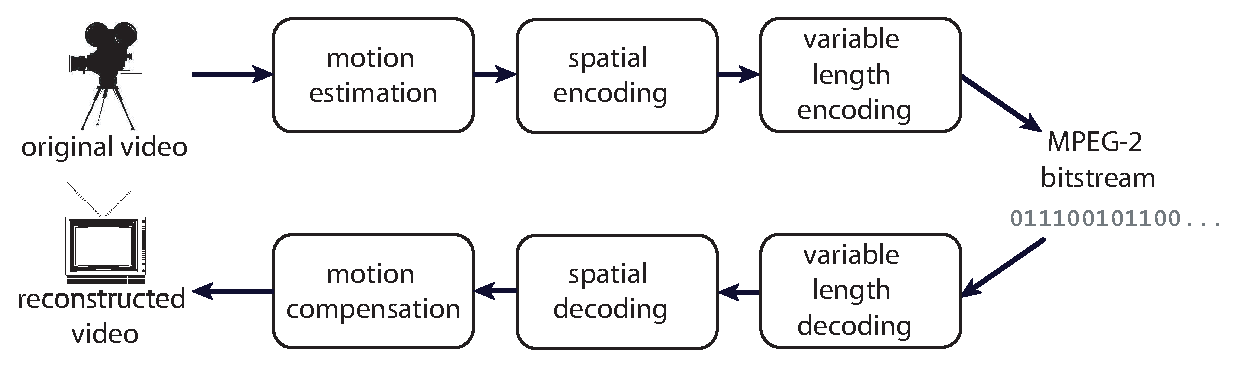
\includegraphics[scale=0.7, angle=0]{./mpeg2_overview.eps}
    \caption{High level view of MPEG-2 decoding and encoding.}
    \label{fig:mpeg2_overview}
  \end{center}
\end{figure}

The MPEG-2 specification contains three types of compression:
variable length coding, spatial coding, and motion prediction.
Figure~\ref{fig:mpeg2_overview} shows a high level overview
of the decoding and encoding process. 
For a complete description of the MPEG-2 data format and coding
scheme one should refer to
the official MPEG-2 standard~\cite{MPEG2}. However, this chapter
contains an abbreviated explanation of the 
standard targeted to a reader lacking prior knowledge of image or video
compression algorithms. The explanation focusses on the 
variable length coding in the parser, 
the functionality needed for spatial coding and decoding,
and the motion prediction components. Iwata et al. estimate that each of these three 
components constitutes a roughly equal portion of the work needed for 
decoding~\cite{iwata98coarse}. Encoding is similar, although
motion estimation constitutes a larger computational effort than
the decoder's motion compensation.

This chapter begins with an enumeration 
of the compression types found in MPEG-2.
It then describes picture organization and the temporal and spatial
transformations that provide compression. 
This is followed by a description of video
organization and finally a list of optional MPEG-2 format extensions.

\section{Compression Techniques}
MPEG-2 uses both {\it lossy} and {\it lossless} compression. 
Lossless compression eliminates redundant information from a signal while allowing
for an exact reconstruction. 
Lossy compression permanently eliminates information from a picture based on
a human perception model. Lossy compression removes details that a casual
observer is likely to miss. A lossy compression is irreversible,
and a lossy decompression process only approximately reconstructs the original
signal. MPEG-2 uses the following compression techniques:

\begin{itemize}
  \item \textbf{Huffman Compression} (\textit{lossless}) 
Huffman compression~\cite{Huffman52} is a form of entropy 
coding. It compresses a signal using variable length codes to efficiently 
represent commonly occurring subpatterns in the signal.
  \item \textbf{Color Channel Downsampling} (\textit{lossy})  
Humans are much better at discerning changes in {\it luminance}, 
than changes in {\it chrominance}. Luminance, or brightness, is a 
measure of color intensity. Chrominance is a measure of color hue.
Pictures are separated into one luminance and two chrominance channels, 
called the \textit{YCbCr} color space. The chrominance channels are
typically downsampled horizontally and vertically. 
  \item \textbf{Frequency Quantization} (\textit{lossy}) 
An image can be expressed as a linear combination of 
horizontal and vertical frequencies.
Humans are much more sensitive
to low frequency image components, such as a blue sky, than to high frequency image components,
such as a plaid shirt. Unless a high frequency component has 
a strong presence in an image, it can be discarded.
Frequencies which must be coded are stored 
approximately (by rounding) rather
than encoded precisely. This approximation process is called
\textbf{quantization}. How the different horizontal and vertical
frequencies are quantized is determined by empirical data
on human perception.
  \item \textbf{Motion Prediction} (\textit{lossless}) 
Frames of a video
contain a great deal of temporal redundancy because much of a
scene is duplicated between sequential frames. Motion estimation is used to
produce motion predictions with respect to one or more reference frames.
Predictions indicate what any given frame should look like. For similar frames, 
only the motion estimate and any error between the predicted values and the
actual values must be encoded.
  \item \textbf{Difference Coding} (\textit{lossless})  
Over any given region in an image the average color value is likely to be
similar or identical to the average color in surrounding regions.
Thus the average colors of regions are coded differentially with respect
to their neighbors. Motion information at neighboring regions is also likely
to be similar or identical and is therefore coded 
differentially with respect to motion at neighboring regions.
\end{itemize}

\section{Picture Organization} 
\label{section:picture_decomp}

\begin{figure}
  \begin{center}
    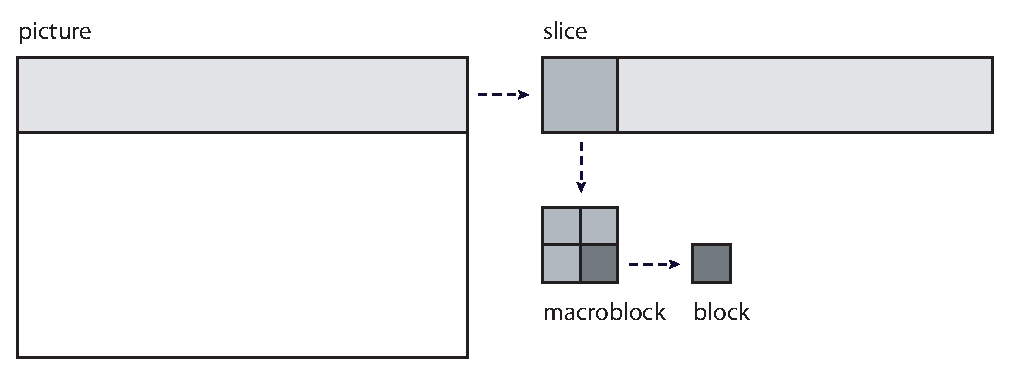
\includegraphics[scale=0.8, angle=0]{./picture_structure.eps}
    \caption{MPEG-2 picture subcomposition.}
    \label{fig:picture_structure}
  \end{center}
\end{figure}

Figure~\ref{fig:picture_structure} shows how the MPEG-2 standard
organizes pictures. Each picture breaks into 
16x16 groups of pixels called \textbf{macroblocks}. 
Adjacent sequences of macroblocks
are contained in a structure called a \textbf{slice}.
Pictures and macroblocks are defined in the
YCbCr color space, and the first step of encoding is
converting the picture into this color representation.

A macroblock is itself composed of 8x8 subpixel 
\textbf{blocks}. There are always
exactly 4 luminance blocks that form a 2x2 array to cover the
macroblock. Because of human insensitivity to chrominance information, each of the two
chrominance channels may be downsampled. 

The type of downsampling in an MPEG-2 stream is called its
\textbf{chroma format}. The two most common chroma formats
are shown in Figure~\ref{fig:chroma_format}. The more common of the two 
is the 4:2:0 format.
This format specifies that each chrominance channel in a macroblock be represented
by a single block, horizontally and vertically
downsampling a macroblock from 16x16 to 8x8 subpixels. 
A 4:2:0 macroblock therefore contains a total of 6 blocks.
An alternate format is 4:2:2. 
The 4:2:2 format uses two blocks for each chrominance 
channel, horizontally downsampling each macroblock from 16x16 to 
8x16 subpixels. 
A 4:2:2 macroblock therefore contains a total of 8 blocks.
A 4:4:4 chroma format also exists but is not commonly used, and specifies 
no color channel downsampling, and uses 4 blocks to 
represent each color channel in a macroblock. 

\begin{figure}
  \begin{center}
    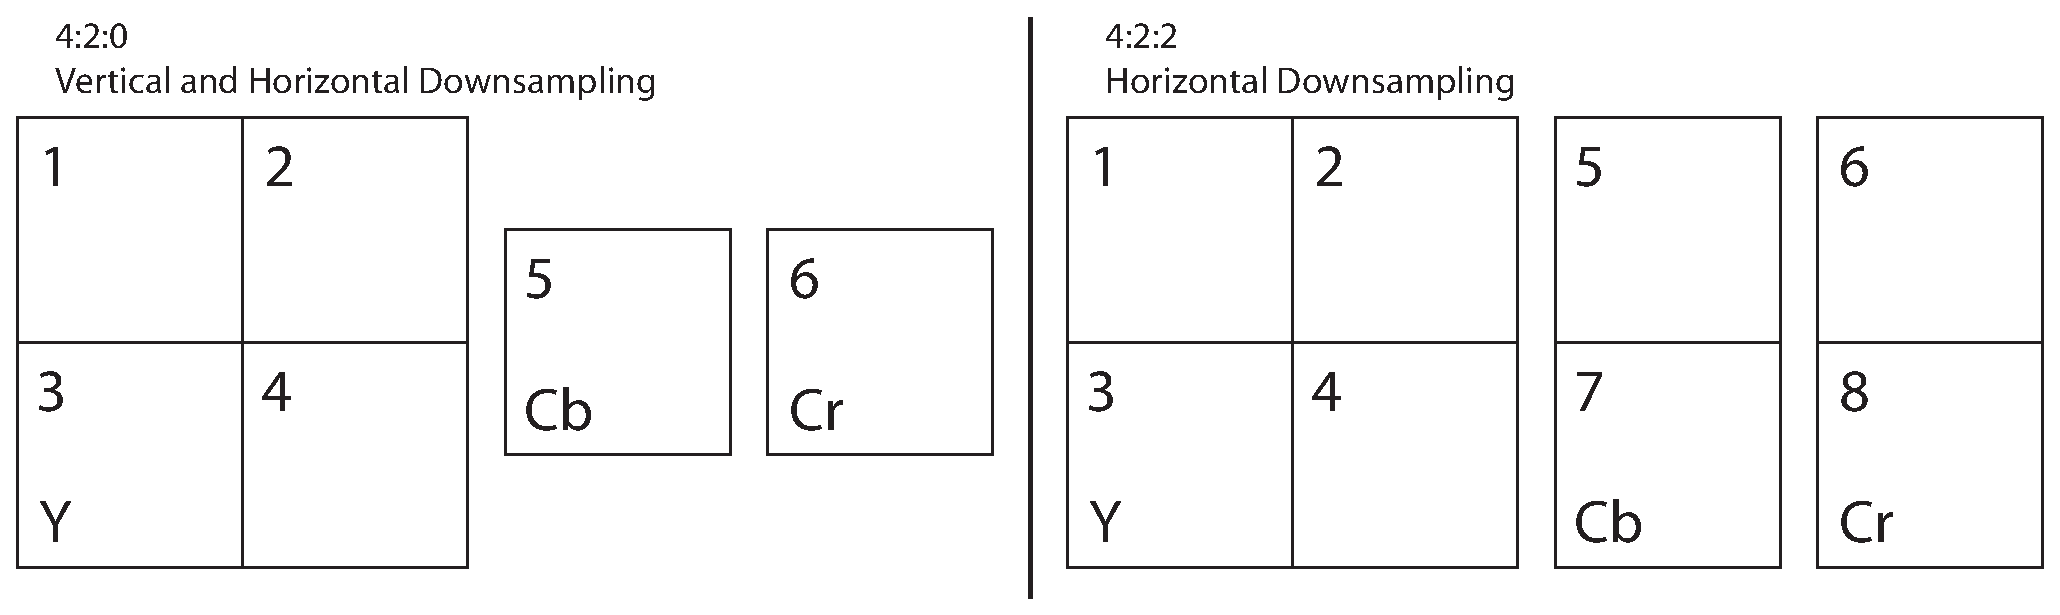
\includegraphics[scale=0.4, angle=0]{./chroma_formats.eps}
    \caption{Commonly used chroma formats.}
    \label{fig:chroma_format}
  \end{center}
\end{figure}

\section{Temporal Compression}

Temporal compression in MPEG-2 is achieved via motion prediction,
which detects and eliminates similarities between macroblocks across
pictures. For any given macroblock $M$, a motion estimator forms a prediction: a \textbf{motion
vector} that contains the horizontal and vertical displacement of that 
macroblock from the most similar macroblock-sized area in one or more reference pictures.
The matching macroblock
is removed (subtracted) from $M$ on a pixel by pixel
basis. The
result is a residual \textbf{predictive coded (P)} macroblock. The residual 
macroblock contains the difference between the motion predicted values for
the macroblock and the macroblock's actual values. A P macroblock
always uses forward motion prediction, meaning that the reference frame
precedes it temporally. (See Section~\ref{subsection:pic_org} for more details on
picture referencing and organization.) Figure~\ref{fig:motion_estimation_forward} illustrates
forward motion estimation.

\begin{figure}[h]
  \begin{center}
    \includegraphics[scale=0.5, angle=0]{./motion_estimation_forward_vectorized.eps}
    \caption{Eliminating temporal redundancy through forward motion estimation.}
    \label{fig:motion_estimation_forward}
  \end{center}
\end{figure}

Macroblocks encoded without the use of motion
prediction are \textbf{intra coded (I)} macroblocks. 
In addition to the forward motion 
prediction used by P macroblocks, it is possible to 
encode new macroblocks using motion
estimation from both temporally previous and subsequent pictures. Such macroblocks
are \textbf{bidirectionally predictive coded (B)} macroblocks, and they exploit a
greater amount of temporal locality. A B macroblock may contain two motion vectors, 
referencing both previous and subsequent pictures; in this case, the 
motion prediction
is an unweighted average of the forward and backward predictions. 
Figure~\ref{fig:motion_estimation_back}
illustrates backward motion estimation.

\begin{figure}[h]
  \begin{center}
    \includegraphics[scale=0.5, angle=0]{./motion_estimation_back_vectorized.eps}
    \caption{Eliminating temporal redundancy through backward motion estimation.}
    \label{fig:motion_estimation_back}
  \end{center}
\end{figure}

All blocks in macroblocks, whether intra coded or residually encoded, undergo 
spatial compression.
Except for the first macroblock in a slice, 
motion vectors are compressed by coding them differentially with respect to the 
motion vectors in the previously decoded 
macroblock\footnote{A second exception is for the first set of
motion vectors following an intra coded macroblock. These vectors 
must always be fully coded because intra coded macroblocks have no motion
vectors.}.

\section{Spatial Compression}
\label{sec:MPEGspatial}

Each block undergoes a two-dimensional \textbf{Discrete Cosine Transform} (DCT),
which is a frequency transform that separates the block into components
with varying visual importance. As shown in Figure~\ref{fig:dct}, 
the DCT takes one 8x8 block as input and produces a 
transformed 8x8 block of frequency coefficients as output. 
Horizontal frequency increases towards the right of the block and
vertical frequency increases towards the bottom of the block.
The upper left corner of the block contains the lowest frequencies
and the lower right corner contains the highest frequencies.

\begin{figure}
  \begin{center}
    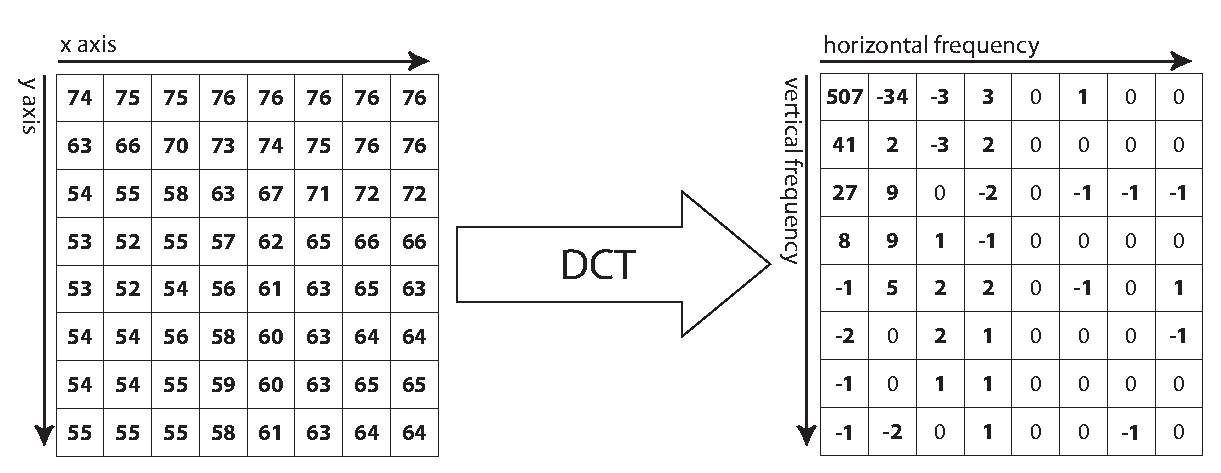
\includegraphics[scale=0.6, angle=0]{./dct.eps}
    \caption{Sample input and output for a discrete cosine transform.}
    \label{fig:dct}
  \end{center}
\end{figure}

The DCT by itself is lossless\footnote{I ignore a possible loss of 
precision, an issue addressed by the MPEG-2 specification and explained
subsequently in Section~\ref{subsection:extra_decoder}}
but enables the quantization of blocks according to a 
\textbf{quantization table} of \textbf{quantization values}, 
also in the frequency domain. The quantization table reflects
a human's relative abilities to discern different frequency
components of an image. 
The quantization table itself may contain any values and can be
specified in the MPEG-2 bitstream, although usually one 
of several standard tables is used.
Each value in a frequency-transformed
block is divided by the corresponding quantization value, with
any remainder thrown away. An example block quantization appears
in Figure~\ref{fig:quantize}\footnote{The quantization process is
technically more complicated than the math I have just described,
although the description is conceptually accurate. The output block
in the figure is accurately quantized, but cannot be arrived at by
the division process I just described.}.
A small error may be introduced
to individual frequency components and most low energy frequency components
are simply reduced to $0$. This stage introduces much of the lossy 
compression in MPEG-2 coding. 

\begin{figure}[h]
  \begin{center}
    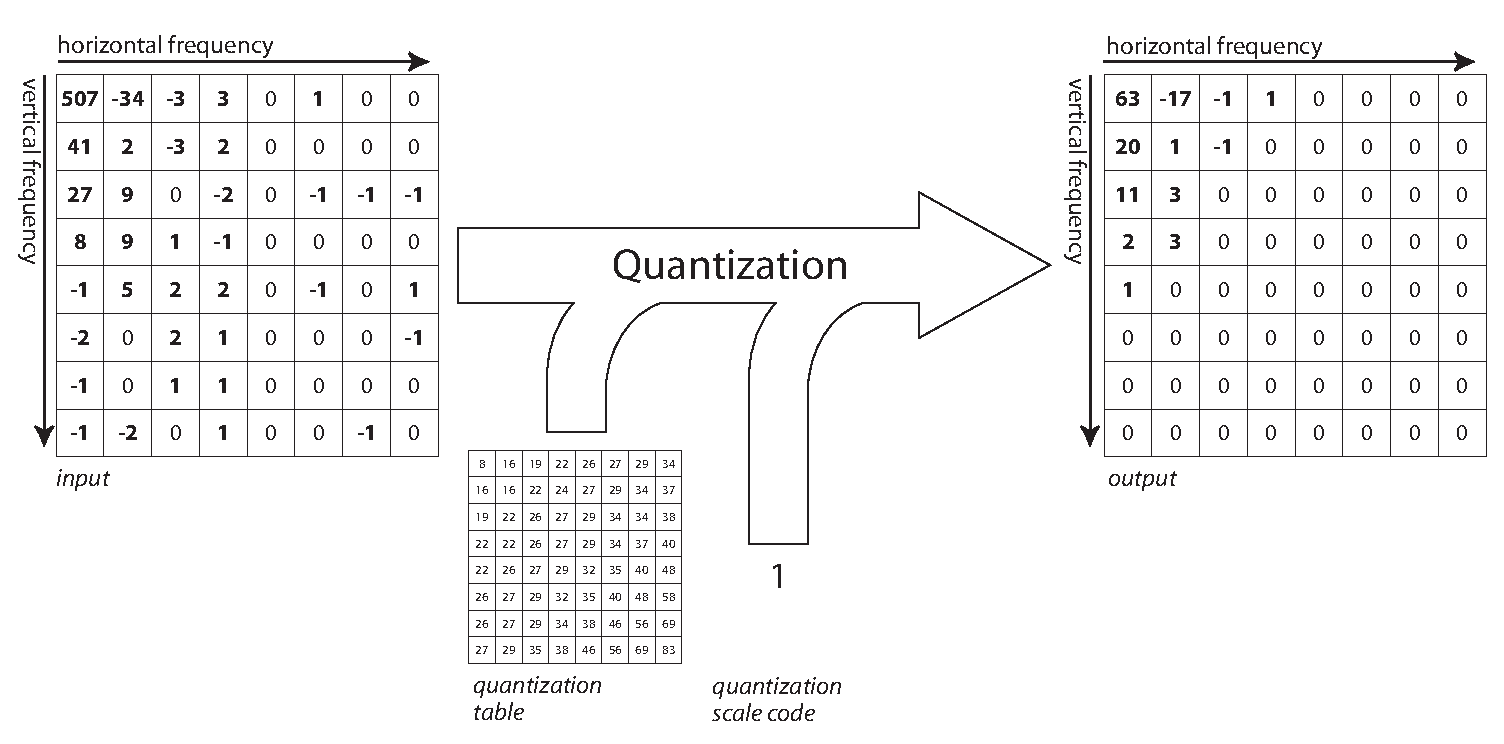
\includegraphics[scale=0.6, angle=0]{./quantization_example2.eps}
    \caption{Example block quantization.}
    \label{fig:quantize}
  \end{center}
\end{figure}

MPEG-2 uses two quantization tables. One table is used for all 
intra coded blocks and the other for residually coded blocks. 
At irregular intervals, an MPEG-2 bitstream indicates a 
\textbf{quantization scale code} which provides an additional 
scaling factor that affects all frequencies in a block. 
One can adjust the desired compression level and
control the video bitrate (bits per second)
by tuning the quantization scale code between macroblocks. 
In an encoder this control 
is typically realized using feedback about the final entropy coded 
output bitrate earlier in the quantization stage.

The upper left value in the frequency transformed block contains the
\textbf{DC coefficient}, which
is the coefficient corresponding to the zero frequency
in both the horizontal and vertical dimensions. Less formally,
this is the average color of the block. 
MPEG-2 differentially encodes the DC block value for 
intra coded blocks. 
The first DC coefficient in the first block in a slice is fully
encoded and all subsequent DC coefficients in a slice are 
differentially coded. Note that the differential coding
semantics for DC coefficients and motion vectors guarantee that
macroblocks in different slices are coded
independently from each other.

After quantization a block is \textbf{zigzag} ordered. 
Zigzag ordering sorts a
block's values from lowest to highest frequency. Since
low-frequency components are more likely to have non-zero 
values following quantization, zigzag ordering consolidates 
non-zero block coefficients together at the beginning of the block. 
The zigzag order commonly used by MPEG-2 is shown in Figure~\ref{fig:zigzag_order}

\begin{figure}
  \begin{center}
    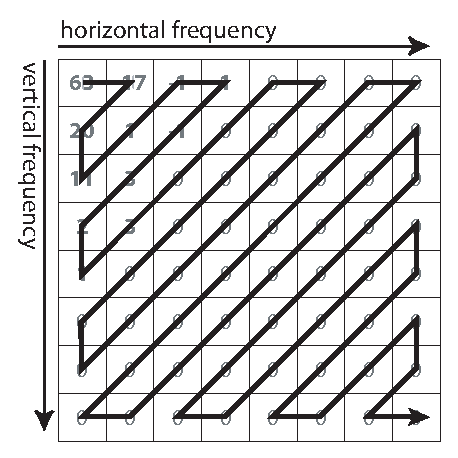
\includegraphics[scale=0.6, angle=0]{./zigzag_order.eps}
    \caption{Zigzag ordering of frequency coefficients from low to high.}
    \label{fig:zigzag_order}
  \end{center}
\end{figure}

The zigzag ordered data is then Huffman compressed using 
a set of predefined Huffman tables defined in the MPEG-2 
specification. Picture metadata, such as the picture type, changes
to the quantization scale code, and motion vectors,
are also Huffman encoded and interleaved in the bitstream.

\section{Required Block Decoding Components}
\label{subsection:extra_decoder}

Data transformation pairs such as a DCT and an inverse DCT (IDCT), may accidentally
introduce loss of data precision, 
due to hardware architecture and algorithm differences 
in a decoder and encoder.
While such imprecisions are tiny, the use of temporal compression
means that small imprecisions accumulate and magnify over the course
of several motion predicted pictures and quickly become noticeable.
For this reason the MPEG-2 specification places specific functional constraints on
mathematical operations in MPEG-2 codecs: 

\begin{itemize}
\item The frequency coefficients emitted from the inverse quantization stage must be saturated within predefined levels.
\item The low-order bit of the highest frequency value in a block is used as a parity bit on the value of the block. In the encoder this bit is set between the DCT and quantization. In the decoder the bit is checked between the saturated inverse quantization and the IDCT. This setting and checking of the bit is called \textbf{mismatch control}.
\item The output of the IDCT is saturated within predefined levels.  
\end{itemize}

\section{Video Organization}

\label{subsection:pic_org}

Just as macroblocks have an associated I, P, or B type, 
pictures also have an associated type, used to 
limit the kinds of macroblocks that they may contain. I pictures 
contain only I macroblocks, P pictures contain I or P macroblocks, 
and B pictures may contain I, P, or B macroblocks. Only I and P 
pictures are used as references for motion prediction and
all I and P pictures are automatically considered references. 
B pictures are never used as references. 

The highest level of organization in an MPEG-2 data stream
is the \textbf{Group of Pictures} (GOP), which 
contains all the information needed to reconstruct a temporally continuous sequence of
video. GOPs consist of I, P, and B pictures.
A typical I:P:B picture ratio in a GOP is 1:3:8, and a typical
picture pattern is a repetition of the following logical sequence,
where the subscripts denote the temporal ordering of the pictures in the video:
\begin{center}
I$_1$~B$_2$~B$_3$~P$_4$~B$_5$~B$_6$~P$_7$~B$_8$~B$_9$~P$_{10}$~B$_{11}$~B$_{12}$~I$_{13}$~$\cdot$~$\cdot$~$\cdot$
\end{center}

Any backwards motion vector in a picture refers to the immediately preceding
reference picture. Likewise, any forward motion vector refers to the subsequent
reference picture. To simplify the decoding process, pictures are not ordered
temporally in the data stream, but rather in the order that they are needed for decoding:
P pictures are always coded with respect to the previous
reference picture and B pictures are always coded with respect to the previous two
reference pictures. Thus, the picture pattern previously described is ordered
in the MPEG-2 data stream as:
\begin{center}
I$_1$~P$_4$~B$_2$~B$_3$~P$_7$~B$_5$~B$_6$~P$_{10}$~B$_8$~B$_9$~I$_{13}$~B$_{11}$~B$_{12}$~$\cdot$~$\cdot$~$\cdot$
\end{center}

\section{Additional MPEG-2 Features}
\label{additional:mpeg}
Because MPEG-2 targets a wide range of devices, the specification is complicated by additional features that make decoding any given video possible on a range of architectures. The following features are mentioned for the sake of completeness, but are excluded from the StreamIt MPEG-2 codec implementations. These features constitute alternative data formats, rather than compression or algorithmic enhancements, and are suitable for exclusion in research-oriented MPEG-2 implementations.

\begin{itemize}
\item \textbf{Interlacing} is a legacy television format needed to support many analog output devices. An interlaced frame contains only half of the original picture data, leaving out alternating horizontal lines. Sequential frames alternate between encoding even and odd scan lines. The alternative to interlacing, which fully encodes each picture, is called \textbf{progressive scan}. 
\item The MPEG-2 bitstream can contain \textbf{layers} which contain alternate encodings of the same picture. A motivating example for this feature is the DVD format, which typically encodes an interlaced version of a movie in the primary layer, and an interlaced version containing the alternate scan lines in a secondary layer. Devices that output interlaced pictures can ignore the secondary layer and devices that output progressive pictures can combine the two layers to produce the complete video.
\item \textbf{Concealment motion vectors} indicate motion estimates for intra-coded macroblocks. These concealment motion vectors are only used to form a macroblock prediction if bitstream errors prevent correct recovery of blocks contained in the macroblock. This plays an important role in the decoding of broadcast MPEG-2 streams such as satellite or HDTV, where transport errors are likely to occur.
\end{itemize}

\section{Related Work}
\label{sec:related}

% BILL

%Signal~\cite{Signal}, 
%Lucid~\cite{Lucid77}, and
%Occam~\cite{Occam}, and Sisal \cite{sisal}.
%Parallel Haskell~\cite{ph}
In addition to StreamIt, there are a number of stream-oriented
languages drawing from domains such as functional, dataflow, CSP and
synchronous programming~\cite{survey97}.  The Brook language is
architecture-independent and focusses on data
parallelism~\cite{brook04}.  Stream kernels are required to be
stateless, though there is special support for reducing streams to a
single value.  Stream\-C/Ker\-nel\-C is lower level than Brook;
kernels written in KernelC are stiched together in StreamC and mapped
to the data-parallel Imagine processor~\cite{imagine03ieee}.  SPUR
adopts a similar decomposition between ``microcode'' stream kernels
and skeleton programs to expose data parallelism~\cite{spur05samos}.
Cg exploits pipeline parallelism and data parallelism, though the
programmer must write algorithms to exactly match the two pipeline
stages of a graphics processor~\cite{cg03}.  Compared to these
languages, StreamIt places more emphasis on exposing task and pipeline
parallelism (all the languages expose data parallelim).
%and on sliding window operations (filters that peek).  
By adopting the synchronous dataflow model of execution~\cite{lee87},
StreamIt focusses on well-structured programs that can be aggressively
optimized.  The implicit infinite loop around programs is also a key
StreamIt characteristic that enables the transformations in this
paper.  Spidle is also a recent stream language that was influenced by
StreamIt~\cite{spidle03}.
%and Lucid Synchrone~\cite{Lucid-Synchrone}.
%Synchronous languages which
%target embedded applications include Esterel~\cite{Esterel},
%Lustre~\cite{Lustre}, and Additional

Liao et al. map Brook to multicore processors by leveraging the affine
partitioning model~\cite{liao06brook}.  While affine partitioning is a
powerful model for parameterized loop-based programs, in StreamIt we
simplify the problem by fully resolving the program structure at
compile time.  This allows us to schedule a single steady state using
flexible, non-affine techniques (e.g., simulated annealing) and to
repeat the found schedule for an indefinite period at runtime.
Gummaraju and Rosenblum map stream programs to a general-purpose
hyperthreaded processor~\cite{gummaraju05micro}.  Such techniques
could be integrated with our spatial partitioning to optimize per-core
performance.  Gu et al. expose data and pipeline parallelism in a
Java-like language and use a compiler analysis to efficiently extract
coarse-grained filter boundaries~\cite{du03sc}.  Ottoni et al. also
extract decoupled threads from sequential code, using hardware-based
software pipelining to distribute the resulting threads across
cores~\cite{ottoni05decoupled}.  By embedding pipeline-parallel
filters in the programming model, we focus on the mapping step.

%%%%%%%%%%%%%%%%%%%%%%%%%%%%%%%%%%%%%%%%%%%%%%%%%%%%%%%%%%%%%%%%%%%%%

Previous work in scheduling computation graphs to parallel targets has
focused on partitioning and scheduling techniques that exploit task
and pipeline parallelism~\cite{SDFSched, SDFSched2,may87communicating,
DAGSched, pipeline-sdf}.  Application of loop-conscious
transformations to coarse-grained dataflow graphs has been
investigated.  Unrolling (or ``unfolding'' in this domain) is employed
for synchronous dataflow (SDF) graphs to reduce the initiation
interval but they do not evaluate mappings to actual
architectures~\cite{unfolding,unfolding2}. Software pipelining
techniques have been applied to SDF graphs onto various embedded and
DSP targets~\cite{bakshi99,chatha-02}, but has required programmer
knowledge of both the application and the architecture. To our
knowledge, none of these systems automatically exploit the combination
of task, data, and pipeline parallelism.  Furthermore, these systems
do not provide a robust end-to-end path for application
parallelization from a high-level, portable programming language.

%% Previous work on instruction-level software pipelining has focused
%% mostly on scheduling machine instructions in a loop via modulo
%% scheduling~\cite{rau81,lam-softpipe}.  The algorithms devised must
%% account for tight resource constraints and complex instruction
%% dependences. Our software-pipelining problem is much less constrained,
%% enabling us to employ a simple greedy heuristic.  

%% Furthermore, a traditional modulo scheduling algorithm is not needed
%% because we have an implicit loop barrier at the end of each
%% steady-state.  ILP compilers for clustered VLIW
%% architectures~\cite{Bulldog,Multiflow,lee98spacetime,qian02} must
%% partition instructions and assign them to clusters as part of the
%% instruction scheduling. Clustering is analogous to our application of
%% filter fusion in our software pipelining algorithm.

\Section{MPEG Decoder in StreamIt}

% TODO: recalculate lines of code using statement count (num of ;)
We implemented an MPEG-2 decoder in StreamIt. It is a fully portable
implementation in that the application is not architecture
dependent. The implementation was carried out by one student
programmer with no prior understanding of MPEG. The development
spanned eight weeks from specification~\cite{MPEG2} to the first fully
functional MPEG decoder. The StreamIt code is nearly 4,921 lines of
code with 48 static streams. The MPEG stream parser is the largest
single filter, consisting of 1,924 lines of code.  The 48 static
streams are compiled to 2,150 filters for a picture resolution of
352x240. In contrast, the reference C
implementation~\cite{reference-mpeg-c} is nearly 9,832 lines of code,
although it provides several features such as interlacing and
multi-layer streams that are not yet implemented in the StreamIt
decoder.

A noteworthy aspect of the StreamIt implementation is its
malleability. We illustrate this using two specific examples.  In the
first example, we focus on the video sampling rates. MPEG-2 streams
are encoded using a 4:2:0 sampling rate, which achieves a 50\%
reduction in the number of bits required to represent a video, with
little noticeable loss of color information. However, better quality
is possible with higher sampling rates since more color information is
retained from the original picture. In this paper, we describe how our
decoder implementation, originally designed to deal with a 4:2:0
sampling rate is modified for a 4:2:2 sampling rate.

In the second example, we describe a straight forward language-level
transformation that exposes the data-parallelism across macroblocks in
a picture. This is done in the context of the decoder pipeline which
consists of the inverse quantization, inverse DCT, and motion
compensator. We show that parallelism can be exposed at various levels
in the decoding process, from macroblock to block granularities, and
that the migration path is trivial.

\Section{Code Malleability: A Case Study}
\label{section:chroma}

To illustrate the concrete benefits of programming in a stream
language, we compare the support for varying chroma formats in the
StreamIt and C implementations.  While the conceptual difference
between chroma formats is merely a change in downsampling ratio, this
leads to a change in the data rates and the ratios of data between the
color channels. This requires that the C implementation parameterize
its buffer sizes, array lengths, array indices, and pointer offsets on
the chroma format; the reference implementation uses a ``chroma flag''
to dictate control flow to alternate index/offset calculations in 43
locations in the code. As an example, a fragment of the
``form\_prediction'' routine (in recon.c~\cite{reference-mpeg-c}) used
for motion compensation is shown in Figure~\ref{fig:chroma}. This
function calls a subroutine to perform the actual motion compensation
on each of the three color channels, passing in array offsets to a
global array holding the data. Lines 4-6 adjusts values used for
address calculations to handle the 4:2:2 and 4:2:0 chroma formats, and
lines 7-9 provide additional adjustments for the 4:2:0 format. While
these offset adjustments are necessary in C, they are difficult for
programmers and make the code hard to understand.

To add support for the 4:2:2 chroma format in our StreamIt decoder, we
modified 31 lines and added 20 new lines. Of the 31 modified lines, 23
were trivial modifications to pass a variable representing the chroma
format as a stream parameter. The greatest substantial change was to
the color channel splitter, previously illustrated on line 20 of
Figure~\ref{fig:dec0with-code}. In the case of a 4:2:2 sampling
rate, the chrominance data, as it appears on the input tape,
alternates between each of the two chrominance channels. Thus, a
nested splitjoin is used to properly recover the appropriate
chrominance channels. The new splitjoin is shown in
Figure~\ref{fig:chroma}.  Even after these modifications, the chroma
format only explicitly dictates control flow in 9 locations. Of
course, the scheduling and buffer management changes dramatically
between chroma formats, but this is automatic and hidden from the
programmer.

\begin{figure*}[t]
 \begin{minipage}[t]{4.3in}
   {
   % Matt's note - this is the C reference code I added.
   % I added the line numbers so I can reference them in the text.
    \begin{scriptsize}
    \begin{verbatim}
1    /* Y */
2    form_component_prediction(src[0]+(sfield?lx2>>1:0),dst[0]+(dfield?lx2>>1:0),
3                              lx,lx2,w,h,x,y,dx,dy,average_flag);
4    if (chroma_format!=CHROMA444)  {
5        lx>>=1; lx2>>=1; w>>=1; x>>=1; dx/=2;
6    }
7    if (chroma_format==CHROMA420)  {
8        h>>=1; y>>=1; dy/=2;
9    }
10   /* Cb */
11   form_component_prediction(src[1]+(sfield?lx2>>1:0),dst[1]+(dfield?lx2>>1:0),
12                             lx,lx2,w,h,x,y,dx,dy,average_flag);
13   /* Cr */
14   form_component_prediction(src[2]+(sfield?lx2>>1:0),dst[2]+(dfield?lx2>>1:0),
15                             lx,lx2,w,h,x,y,dx,dy,average_flag);    
    \end{verbatim}
    \end{scriptsize}
   }
   % \vspace{-3pt}
   % \caption{Decoding stream to handle 4:2:0 and 4:2:2 chroma formats.}
   % \label{fig:chroma-stream}
  \end{minipage}
    ~~\hrule~~
 \begin{minipage}[t]{4.3in}
   {
    \begin{scriptsize}
    \begin{verbatim}
    // C = blocks per chrominance channel per macroblock 
    // C = 1 for 4:2:0, C = 2 for 4:2:2
    add splitjoin {
      split roundrobin(4*(B+V), 2*C*(B+V));
      add MotionCompensation() to PT1;
      add splitjoin {
        split roundrobin(N, N);
        for (int i = 0; i < 2; i++) {
          add MotionCompensation() to PT1;
          add ChannelUpsample(C);
        }
        join roundrobin(1, 1);
      }
      join roundrobin(1, 1, 1);
    }
    \end{verbatim}
    \end{scriptsize}
   }
   % \vspace{-3pt}
   % \caption{Decoding stream to handle 4:2:0 and 4:2:2 chroma formats.}
   % \label{fig:chroma-stream}
  \end{minipage}
  ~~\vrule~~
  \begin{minipage}[t]{2.0in}
  {
   \begin{center}
    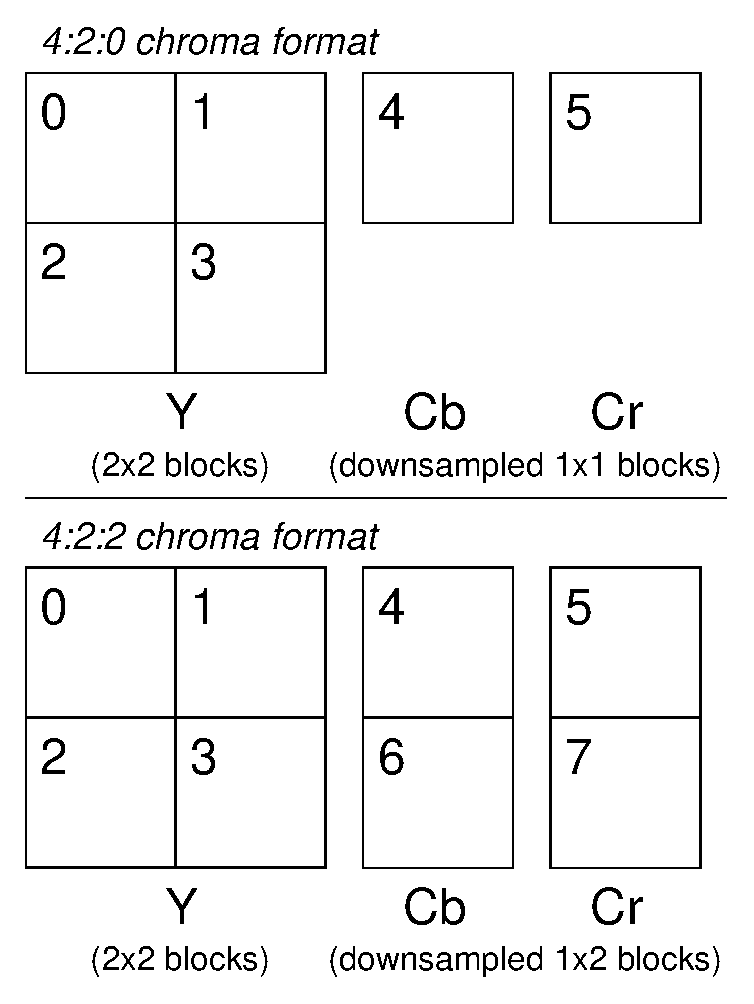
\epsfig{file=chroma_format.eps, width=2.5in}
    % \caption{4:2:0 and 4:2:2 chroma formats showing macroblock ordering}
    % \label{fig:chroma-format}
   \end{center}
  }
  \end{minipage}
  \caption{Decoding stream to handle 4:2:0 and 4:2:2 chroma
    formats. Figures on right illustrate how macroblock orderings
    differ.}
  \label{fig:chroma}
\end{figure*}

\SubSection{Motion Compensation}

An MPEG decoder accepts a bitstream as input and performs Huffman and
variable run-length decoding (VLD).  This process results in a set of
quantized, frequency-domain macroblocks and corresponding motion
vectors.  The decoder inverse quantizes (IQ) the macroblocks and then
performs an inverse DCT (IDCT) to convert the macroblocks to the
spatial domain.  For predictively coded macroblocks (e.g., P and B
pictures), the decoder performs motion compensation (MC) using the
input motion vectors to find a corresponding macroblock in a
previously decoded, stored reference picture. This reference
macroblock is added to the current macroblock to recover the original
picture data. If the current macroblock is part of an I or P picture,
then the decoder stores it for future reference.
Figure~\ref{fig:dec_block} illustrates the decode sequence.

\begin{figure}[htbp]
\centerline{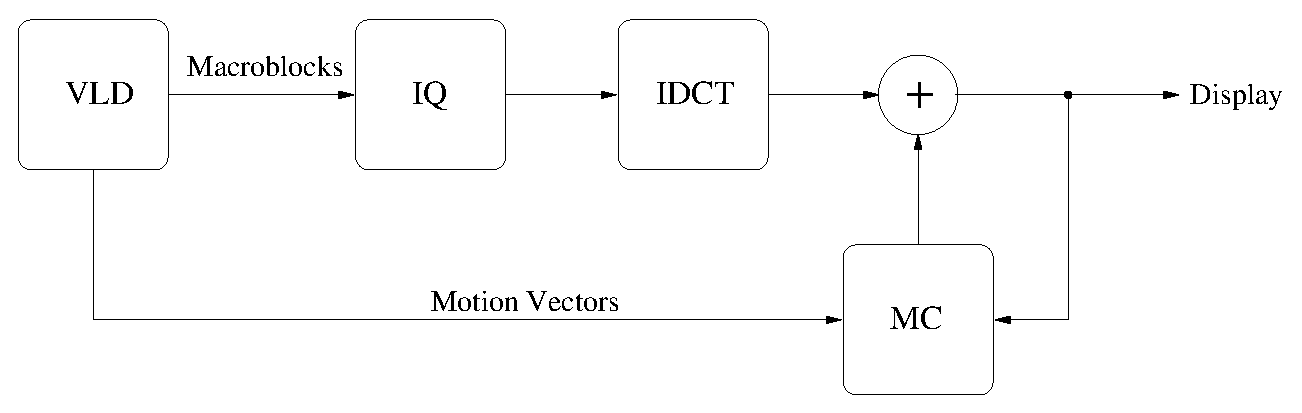
\epsfig{file=dec_block.eps,width=5in}}
\caption{Block diagram of MPEG-2 decode.}
\label{fig:dec_block}
\end{figure}

A simple strategy for parallelizing the MPEG-2 decoding can exploit
the data parallelism among macroblocks. Using this scheme, the Huffman
and run-length decoding is inherently serial, as macroblock boundaries
can only be discovered by performing the decode operation.  Once this
decode is complete, a parallel implementation can distribute
macroblocks to independent streams (using a splitjoin). Each stream
performs the inverse quantization, inverse discrete cosine transform,
and motion compensation. Furthermore, each stream locally stores
reference macroblocks for future motion compensation. Using this
strategy, the streams can execute independently with one exception.

% TODO: This is the figure showing the macroblock parallelism
% I'm not sure where it goes. - Matt
\begin{figure*}[t]
\vspace{-12pt}
%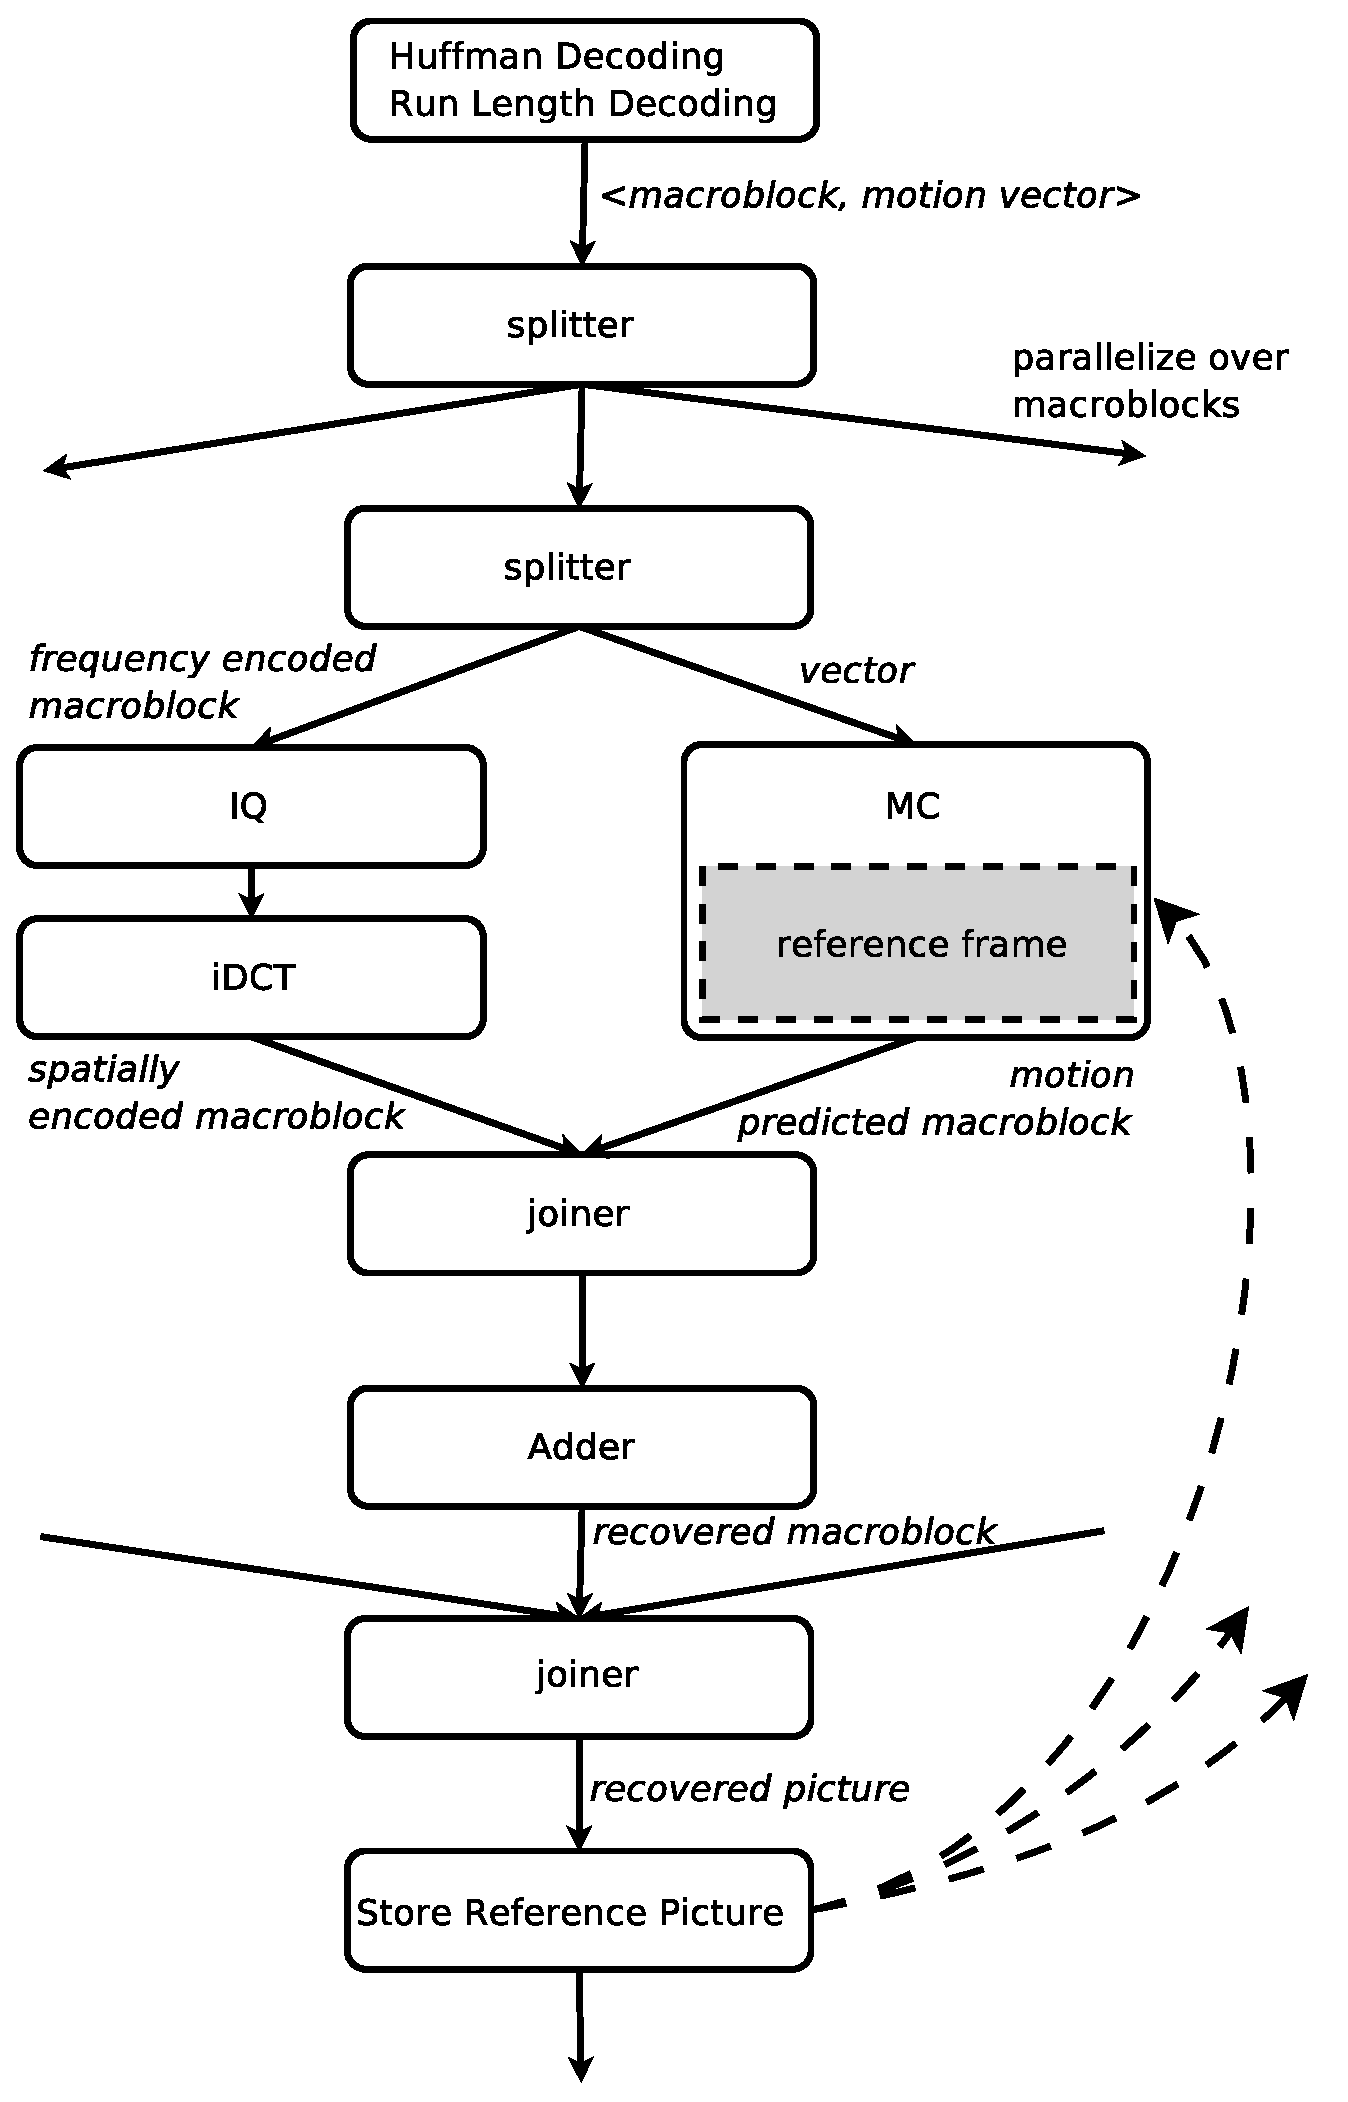
\epsfig{file=decoder_macroblock_parallelism.eps, width=3in}
%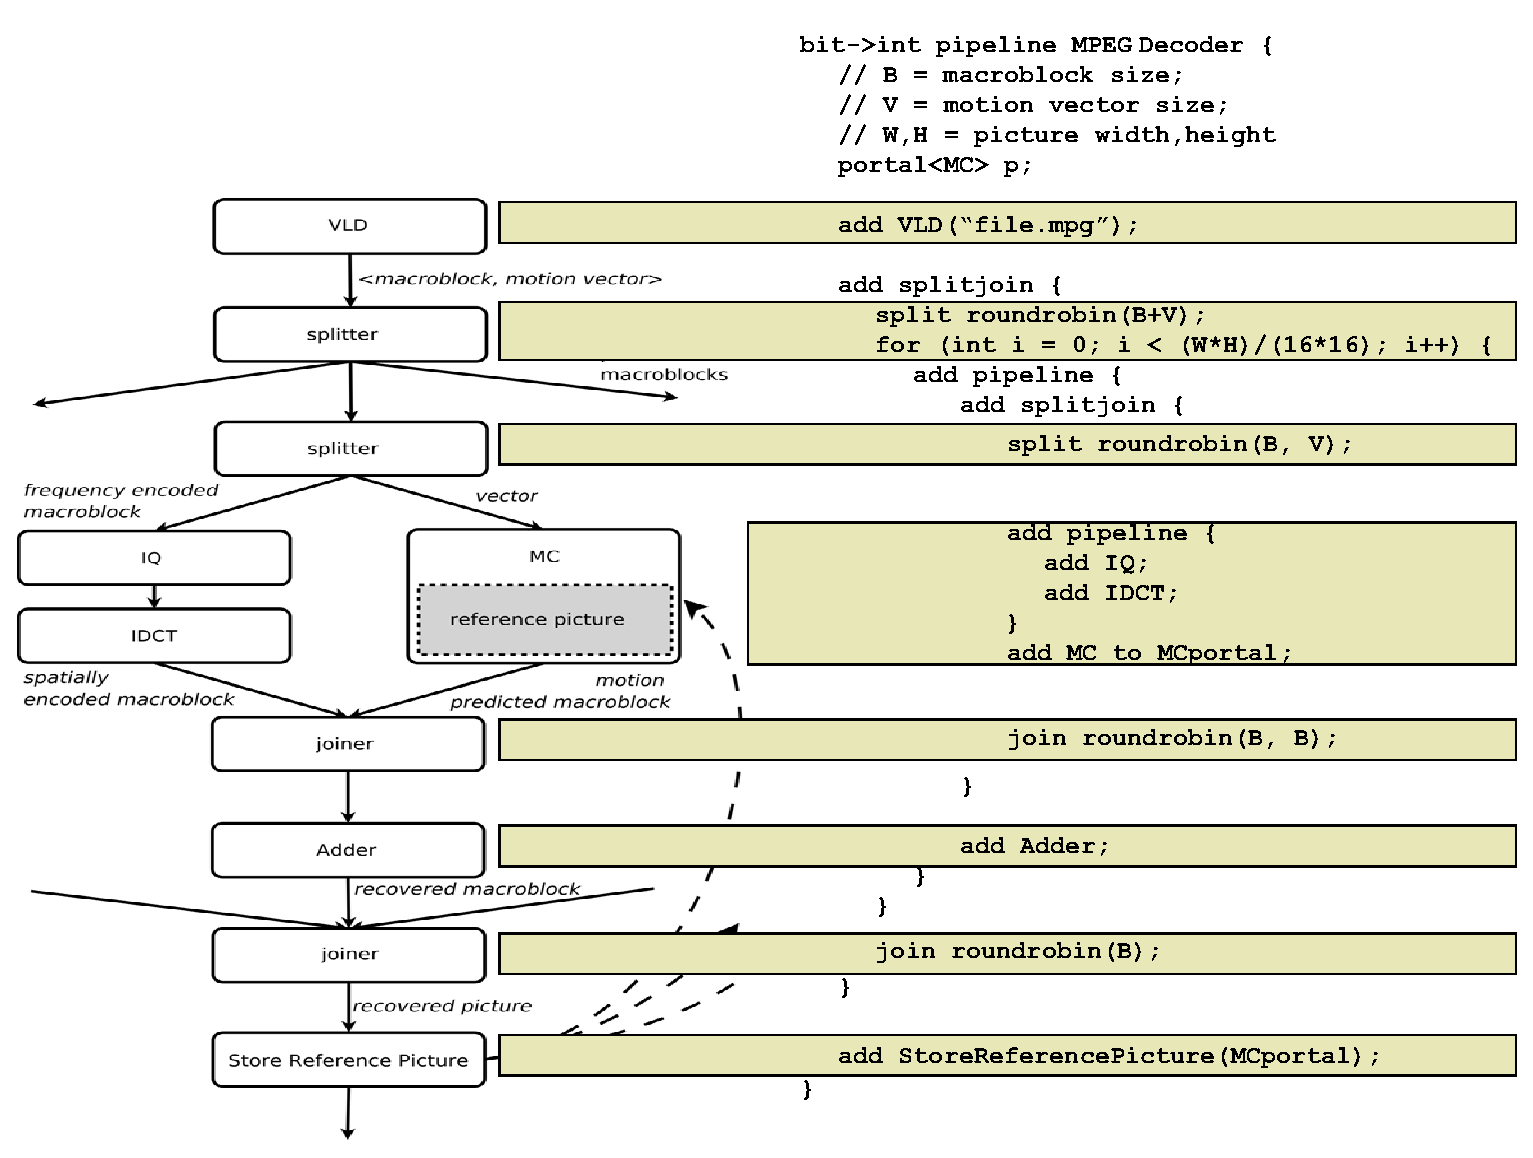
\epsfig{file=decoder-parallel.eps, width=\textwidth}
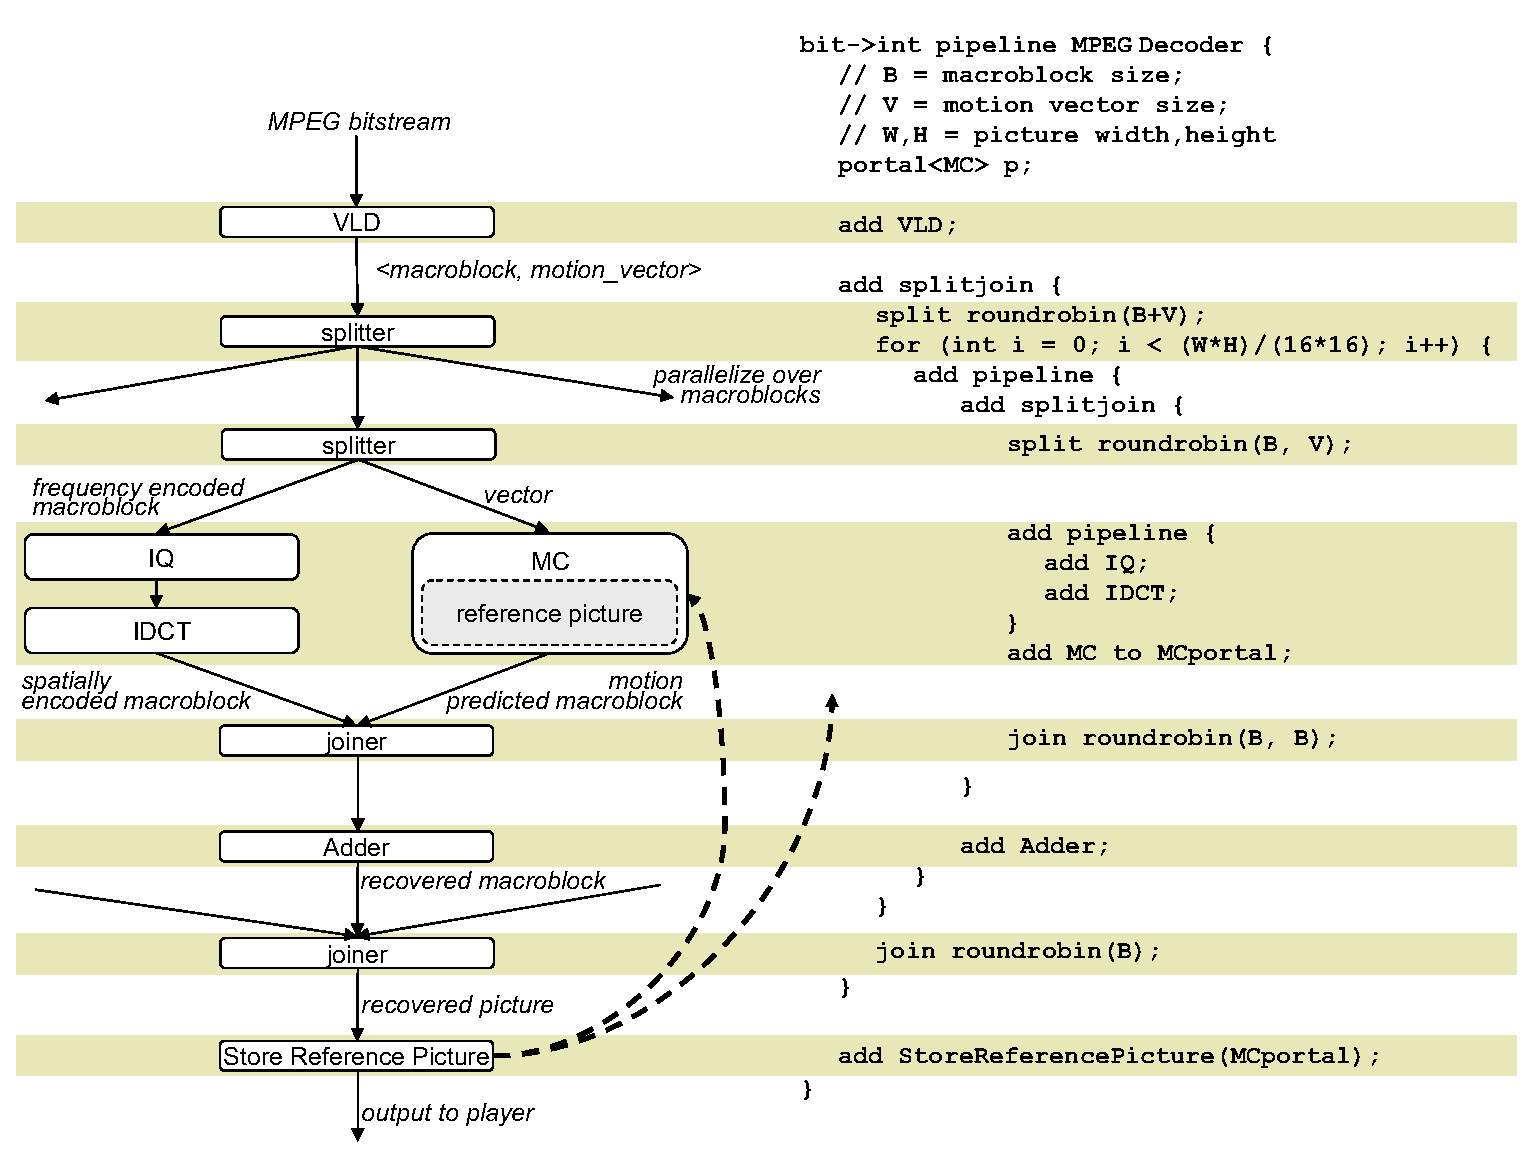
\epsfig{file=decoderpipeline.eps, width=\textwidth}
% TODO: Change Matt's 2 am caption.
\caption{MPEG-2 decoder exploiting macroblock-level parallelism.}
\label{decoder_macroblock_parallelism}
\vspace{-6pt}
\end{figure*}

This exception occurs when a stream is performing motion compensation
and the corresponding motion vector indicates a reference macroblock
stored in some other stream. In this case, inter-stream communication
is required to send the reference data to the requesting stream. This
situation is not uncommon, and is more prevalent for higher resolution
pictures. A simple scheme for handling this situation is for every
stream to broadcast its decoded macroblocks to all other streams. This
solution has the benefit of being conceptually easy to understand and
implement. StreamIt allows programmers to naturally expose such
parallelism. A StreamIt pipeline that operates at macroblock
granularity is shown in Figure~\ref{decoder_macroblock_parallelism}. It is
worthy to note that there is a high correlation between the stream
graph, and the StreamIt syntax describing the pipeline.

The implementation can be made more fine grained by exposing the
intra-macroblock parallelism. For example, the IQ-IDCT pipeline can
operate at a block level, rather than at a macroblock
granularity. This is easily achieved by encapsulating the IQ-DCT pipeline
within a splitjoin to scatter the blocks, operate, and gather the
results to recover the parent macroblock.

There are many implementation strategies for the decoder, each with
varying degrees of exposed parallelism. Of the greatest advantage of
the StreamIt implementation is its malleability. The stream graph is
easily reconfigured to operate at picture-level granularity (exposing
parallelism between chroma channels), macroblock level (exposing even
more data-level parallelism), or even at block level (exposing the
greatest amount of data-level parallelism). The modularity of the
language also affords the ability to cleanly define stream interfaces,
and reuse existing components. As an example, the zig-zag descrambler,
inverse quantizer, and inverse DCT components were all reused for our
JPEG codec implementation. The modularity also reduces the complexity
of the debugging process, as stream components can be functionally
verified independently, leading to greater programmer productivity.

%% TODO: add figure showing decoder pipeline at macroblock granularity
%% and streamit text ala Bill's beamformer/fmradio examples



\chapter{Programmability and Productivity}
\label{chapter:compare}

As previously mentioned, the StreamIt language aims to improve 
programmability for streaming applications. This chapter expands 
on this topic by giving specific instances from the MPEG-2 codec 
implementations where StreamIt improved programmer productivity.

Section~\ref{sec:buffer_management} focusses on StreamIt's 
implicit buffer management. Section~\ref{sec:pipelines_block}
describes how pipelines preserve the block diagram structure
in the program definition and provide a one-to-one mapping with
code. Sections~\ref{sec:expose_data}~and~\ref{section:chroma}
show StreamIt's ability to expose data distribution and
how this leads to a high degree of malleability. 
Section~\ref{sec:hier} describes the advantages of
hierarchical stream graph construction and 
Section~\ref{sec:teleport_useful} the advantages of 
teleport messaging.

Because I particularly want to contrast with 
traditional languages, a number of C code comparisons appear in 
this and the subsequent section. These code examples come from the 
C reference decoder implementation~\cite{reference-mpeg-c} provided 
by the MPEG Software Simulation Group and used in the 
MediaBench~\cite{lee97mediabench} benchmark suite. Because our 
StreamIt code does not support interlacing or certain optional 
bitstream semantics, I have modified the C reference implementation 
to remove that additional functionality, for the purposes of fair 
comparison. The comparison is between the StreamIt decoder of $2282$ 
lines, and the C reference code of $3477$ lines\footnote{As before, line counts 
were generated using \texttt{SLOCcount}~\cite{sloccount}.}. 
I believe this line count comparison is a fair 
quantization of StreamIt's ability to concisely express the MPEG-2 
decoder computations.

\section{Buffer Management}
\label{sec:buffer_management}

\begin{figure}
  \begin{center}
    \begin{minipage}{4in}
      \begin{small}
        \begin{verbatim}
01 static void Add_Block(comp,bx,by)
02      int comp,bx,by;
03 {
04   int cc,i, j, iincr;
05   unsigned char *rfp;
06   short *bp;
08   cc = (comp<4) ? 0 : (comp&1)+1;
09   if (cc==0) {
10     rfp = current_frame[0] + 
11           Coded_Picture_Width*(by+((comp&2)<<2)) + 
12           bx + 
13           ((comp&1)<<3);
14     iincr = Coded_Picture_Width - 8;
15     if (chroma_format!=CHROMA444)
16       bx >>= 1;
17     if (chroma_format==CHROMA420)
18       by >>= 1;
19     rfp = current_frame[cc] + 
20           Chroma_Width*(by+((comp&2)<<2)) + 
21           bx + 
22           (comp&8);
23     iincr = Chroma_Width - 8;
25   }
26   bp = ld->block[comp];
27   for (i=0; i<8; i++) {
28     for (j=0; j<8; j++) {
29       *rfp = *bp++ + *rfp;
30       rfp++;
31     }
32     rfp+= iincr;
33   }
34 }
        \end{verbatim}
      \end{small}
    \end{minipage}
  \end{center}
  \caption{Combining the spatially and temporally decoded data in C.}
  \label{fig:add-filter-in-c}
\end{figure}

\begin{figure}
  \begin{center}
    \begin{minipage}{3in}
      \begin{small}
        \begin{verbatim}
01 int->int filter Add_Block {
02   work pop 2 push 1 {
03     push(pop()+pop());
04   }
05 }
        \end{verbatim}
      \end{small}
    \end{minipage}
  \end{center}
  \caption{Combining the spatially and temporally decoded data in StreamIt.}
  \label{fig:add-filter2}
\end{figure}

Figure~\ref{fig:add-filter-in-c} shows the C code responsible for merging the
spatially and temporally decoded block data\footnote{The original Add\_Block function
performed some unrelated parts of the decoding process as well and was almost 99 lines
long. For comparison purposes the unrelated code is removed.}. Prior to the execution of this
function the IDCT function has generated the motion prediction
error and the motion compensation function has generated the motion prediction. 
These two sets of data are summed to produce the decoded blocks.

Lines 9 through 25 determine the appropriate memory addresses 
for the next block to be processed. Lines 26 to 33 perform the
summation.
Note that line 29 is the only line actually performing the summation. 
The buffer management details dominate every line of code and obscure its functional
purpose. 
The buffer management details are particularly complicated
because the address of the data is dependent on the block's position in a picture,
the size of the video, and the chroma format. The complicated arithmetic
used to adjust buffer indices will make it challenging for a compiler to extract
parallelism. Further complicating any compiler analysis is the function's reuse
 of an input buffer as an output buffer (as reflected in
line 29). 

Reusing buffers is one of many buffer management strategies. The strategy yielding
the best performance depends on the 
target architecture and the size of the buffer. However, the programmer has been
forced to guess about the performance and commit to a particular strategy. 
Also note that a programmer using this function must manually determine 
an execution schedule and buffer sizes that avoid buffer underflow or the premature
overwriting of data.

Now consider the equivalent StreamIt code for adding the decoded block data, shown in
Figure~\ref{fig:add-filter2}. The code itself is almost trivial. The filter 
occurs after a \texttt{roundrobin(1)} joiner merging the prediction error
and the prediction itself. Figure~\ref{fig:motion_prediction_parallel}, 
explained in detail later in Chapter~\ref{chapter:exposing_parallelism}, shows
this filter in the context of the motion compensation stream graph. Note that 
the amount of data this filter processes will 
be dependent on the same chrominance and picture size parameters as the C code
but the buffer management details are hidden from the programmer - they will
be reflected in the data rates of the splitters and joiners surrounding
the filter in the motion compensation graph. At compile
time the compiler makes the decisions about the best buffer management 
strategy~\cite{sermulins05lctes}.  

\section{Pipelines Preserve Block Structure}
\label{sec:pipelines_block}

The pipeline construct preserves the structure implicit in a block diagram.
Figure~\ref{fig:spatial_decoding1} shows a block diagram for spatial decoding
taken from Figures 7-1 and 7-4 of the MPEG-2 specification~\cite{MPEG2}.
Figure~\ref{fig:spatial_decoding0} shows the 
StreamIt code that implements the pipeline. The obvious 
correspondence points to StreamIt's ability to naturally
represent this computation. Note that the quantization
parameters in the diagram are realized as messages in the stream graph.

\begin{figure}[h]
  \center{
    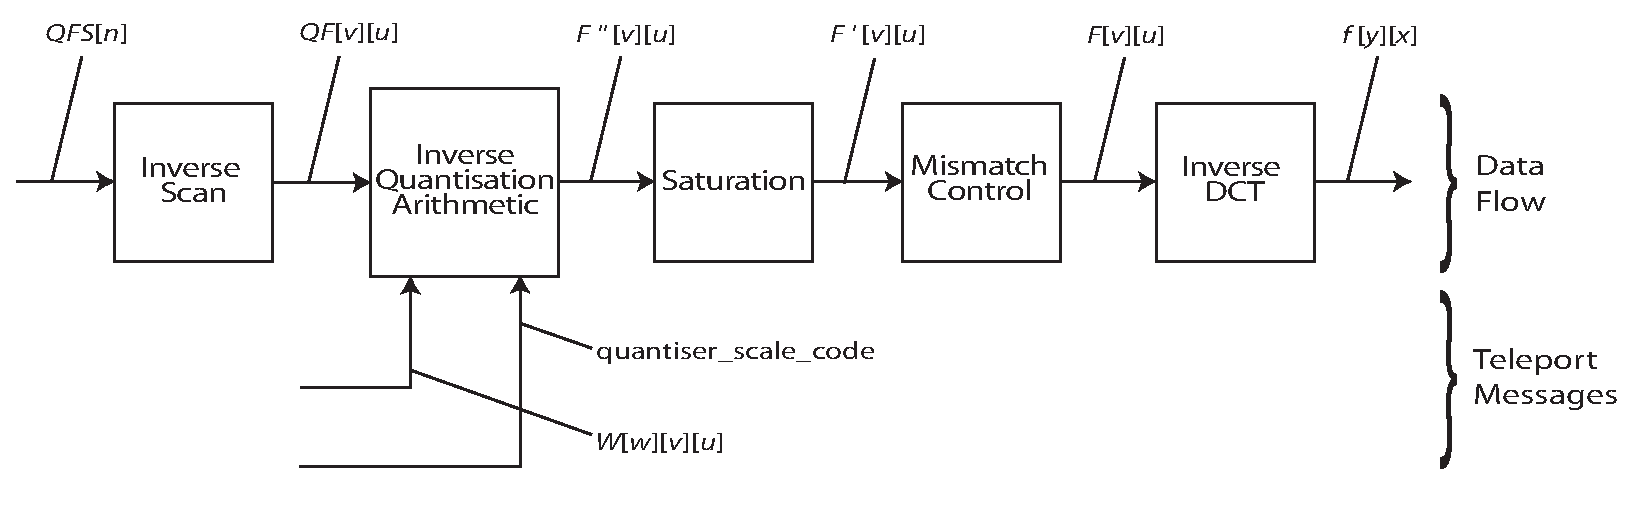
\includegraphics[scale=0.55, angle=0]{./block_decoding.eps}
    \vspace{-12pt}
 	\caption{Block diagram for spatial decoding (from MPEG-2 specification).}
 	\label{fig:spatial_decoding1}
  }
\end{figure}

\begin{figure}
  \begin{center}
    \begin{minipage}{3.5in}
      \begin{small}
        \begin{verbatim}
int->int pipeline BlockDecode(
  portal<InverseQuantization> quantiserData,
  portal<MacroblockType> macroblockType) {

  int[64] Order = {...};
  add ZigZag(64, Order);
  add InverseQuantization() to quantiserData,
                               macroblockType;
  add Saturation(-2048, 2047);
  add MismatchControl();
  add 2D_iDCT(8); // 8x8 2D IDCT
  add Saturation(-256, 255);

}
        \end{verbatim}
      \end{small}
    \end{minipage}
  \end{center}
 	\caption{StreamIt pipeline for spatial decoding.}
 	\label{fig:spatial_decoding0}
\end{figure}

An important detail to note is that each of the filters used in a pipeline
may have different granularities. In this case 
the inverse scan, quantization, and IDCT all operate on blocks of 64 data
values at a time. The mismatch control and saturation blocks are naturally expressed
in terms of a single input and output token. Nowhere must the programmer specify
the number of executions or the execution sequence needed to fully decode a picture
or video. This granularity variance holds through the rest of MPEG-2 as well.
Picture reordering can be expressed in terms of pictures and motion compensation in terms of motion vectors. 
The programmer's burden is eased since he does not have to worry about the rate discrepancies
between filters. 

\section{Natural Exposure of Data Distribution}
\label{sec:expose_data}

\begin{figure}
  \begin{center}
    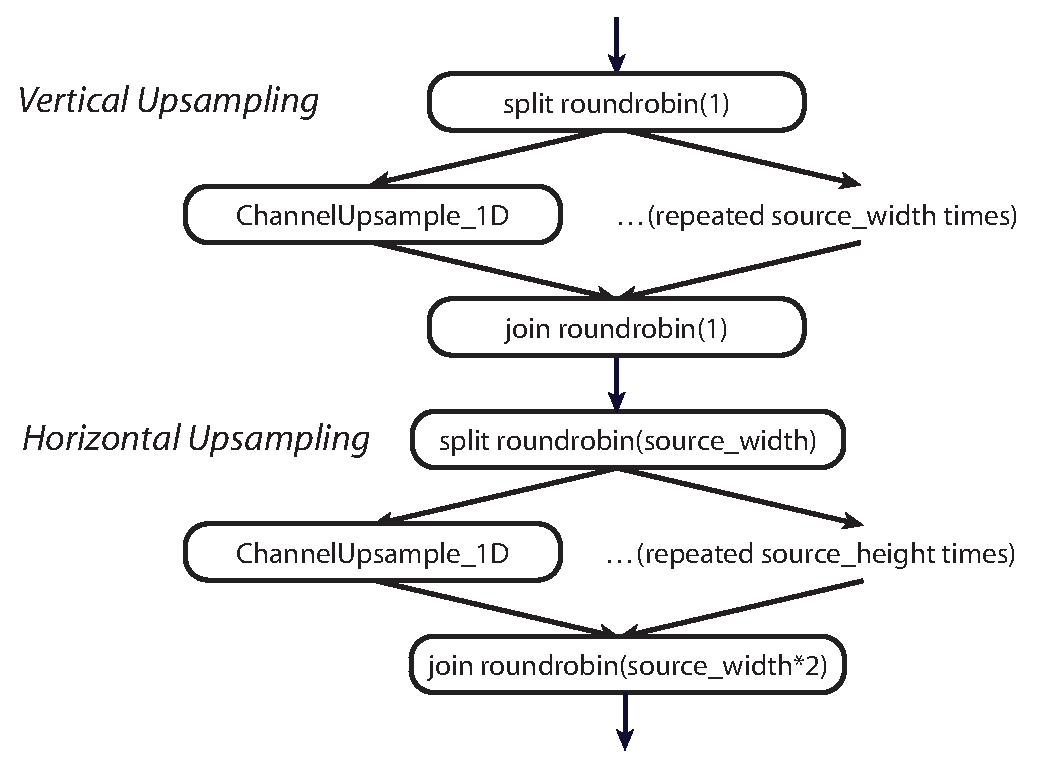
\includegraphics[scale=0.6, angle=0]{./channel_upsampling.eps}
    \caption{2D upsampling decomposed into 1D upsampling}
    \label{fig:how-upsampler-splits-data}
  \end{center}
\end{figure}

\begin{figure}
  \begin{center}
    \begin{minipage}{5.2in}
      \begin{small}
        \begin{verbatim}
int->int splitjoin ChannelUpsample_Vertical(int sourcewidth, 
                                            int sourceheight) {
    split roundrobin(1);
    for (int i = 0; i < sourcewidth; i++) {
        add ChannelUpsample_1D(sourceheight, 0.75, 0.25);
    }
    join roundrobin(1);
}

int->int splitjoin ChannelUpsample_Horizontal(int sourcewidth, 
                                              int sourceheight) {
    split roundrobin(sourcewidth);
    for (int i = 0; i < sourceheight; i++) {
        add ChannelUpsample_1D(sourcewidth, 0.5, 0.5);
    }
    join roundrobin(sourcewidth*2);
}
        \end{verbatim}
      \end{small}
    \end{minipage}
  \end{center}
  \caption{Splitjoins for channel upsampling.}
  \label{fig:upsamplecode}
\end{figure}

The splitjoin construct is a robust mechanism for expressing 
parallelism and data reordering operations. It can be used 
to specify coarse grained parallelism at the highest levels 
of an application because it exposes the independence of computational 
blocks. But it is also useful for describing how a 
computation should be performed, exposing 
coarse grained and fine grained parallelism 
as a byproduct. 

Channel upsampling illustrates this. One can easily 
think of 2D upsampling in terms of 1D upsampling in the vertical 
and horizontal direction\footnote{This is conceptually similar
to the decomposition of a 2D DCT, discussed 
later in Section~\ref{sec:2d_dct}. 
In this case the channel upsampling represents a smaller
amount of work and the splitjoin is more interesting for its
ability to efficiently express the transformation than its ability
to expose parallelism.}. The 
natural way to express upsampling a picture in either 
direction is as a parallel computation on every row or 
column of the picture. The building block is a one-dimensional 
upsampling filter that takes in a pair of weights used for 
interpolation between points. The weights are different for 
horizontal and vertical upsampling because MPEG-2 downsamples 
horizontally by removing pixels, and vertically by displacing 
them. 
The vertical upsampler splits the 
data by column and the horizontal upsampler splits the data 
by row. Figure~\ref{fig:how-upsampler-splits-data} illustrates 
the procedure and Figure~\ref{fig:upsamplecode} shows the 
StreamIt code that implements the process. The C reference
implementation implements upsampling as a series of loops
wrapped around a one dimensional upsampling kernel. In this
case the code looks similar to the StreamIt code. However,
the StreamIt \texttt{for} loops represent graph topology
resolved at initialization time. The C compiler must analyze
the body of the loops to extract parallelism.

\section{Code Malleability}
\label{section:chroma}

\begin{figure}
\begin{center}
  \begin{minipage}[t]{4.8in}
    \begin{small}
      \begin{verbatim}
   /* Y */
01 form_component_prediction(src[0]+(sfield?lx2>>1:0),
02                           dst[0]+(dfield?lx2>>1:0),
03                           lx,lx2,w,h,x,y,dx,dy,average_flag);
04 if (chroma_format!=CHROMA444)  {
05    lx>>=1; lx2>>=1; w>>=1; x>>=1; dx/=2;
06 }
07 if (chroma_format==CHROMA420)  {
08   h>>=1; y>>=1; dy/=2;
09 }
   /* Cb */
10 form_component_prediction(src[1]+(sfield?lx2>>1:0),
11                           dst[1]+(dfield?lx2>>1:0),
12                           lx,lx2,w,h,x,y,dx,dy,average_flag);
   /* Cr */
13 form_component_prediction(src[2]+(sfield?lx2>>1:0),
14                           dst[2]+(dfield?lx2>>1:0),
15                           lx,lx2,w,h,x,y,dx,dy,average_flag);    
      \end{verbatim}
    \end{small}
  \end{minipage}
  \caption{C code excerpt for handling
           4:2:0 and 4:2:2 chroma formats.}
  \label{fig:chroma-format-code-C}
\end{center}
\end{figure}

\begin{figure}
\begin{center}
  \begin{minipage}[t]{3.5in}
    \begin{small}
      \begin{verbatim}
// B = amount of data per block
// V = amount of data per motion vector
add splitjoin {
  split roundrobin(4*(B+V), B+V, B+V);
  add MotionCompensation(4*(B+V)) to PT1;
  for (int i = 0; i < 2; i++) {
    add pipeline {
      add MotionCompensation(B+V) to PT1;
      add ChannelUpsample(B);
    }
  }
  join roundrobin(1, 1, 1);
}
      \end{verbatim}
    \end{small}
  \end{minipage}
  \caption{Original StreamIt code excerpt for handling
           4:2:0 chroma format only.}
  \label{fig:chroma-format-code-streamit-previous}
\end{center}
\end{figure}

\begin{figure}
\begin{center}
  \begin{minipage}[t]{3.5in}
    \begin{small}
      \begin{verbatim}
// C = blocks per chroma channel 
//     per macroblock 
// C = 1 for 4:2:0, C = 2 for 4:2:2
// B = amount of data per block
// V = amount of data per motion vector
add splitjoin {
  split roundrobin(4*(B+V), 2*C*(B+V));
  add MotionCompensation(4*(B+V)) to PT1;
  add splitjoin {
    split roundrobin(B+V, B+V);
    for (int i = 0; i < 2; i++) {
      add pipeline {
        add MotionCompensation(B+V) to PT1;
        add ChannelUpsample(C*B);
      }
    }
    join roundrobin(1, 1);
  }
  join roundrobin(1, 1, 1);
}
      \end{verbatim}
    \end{small}
  \end{minipage}

  \caption{StreamIt code excerpt for handling
           4:2:0 and 4:2:2 chroma formats.}
  \label{fig:chroma-format-code-streamit}
\end{center}
\end{figure}

\begin{figure}
  \begin{center}
    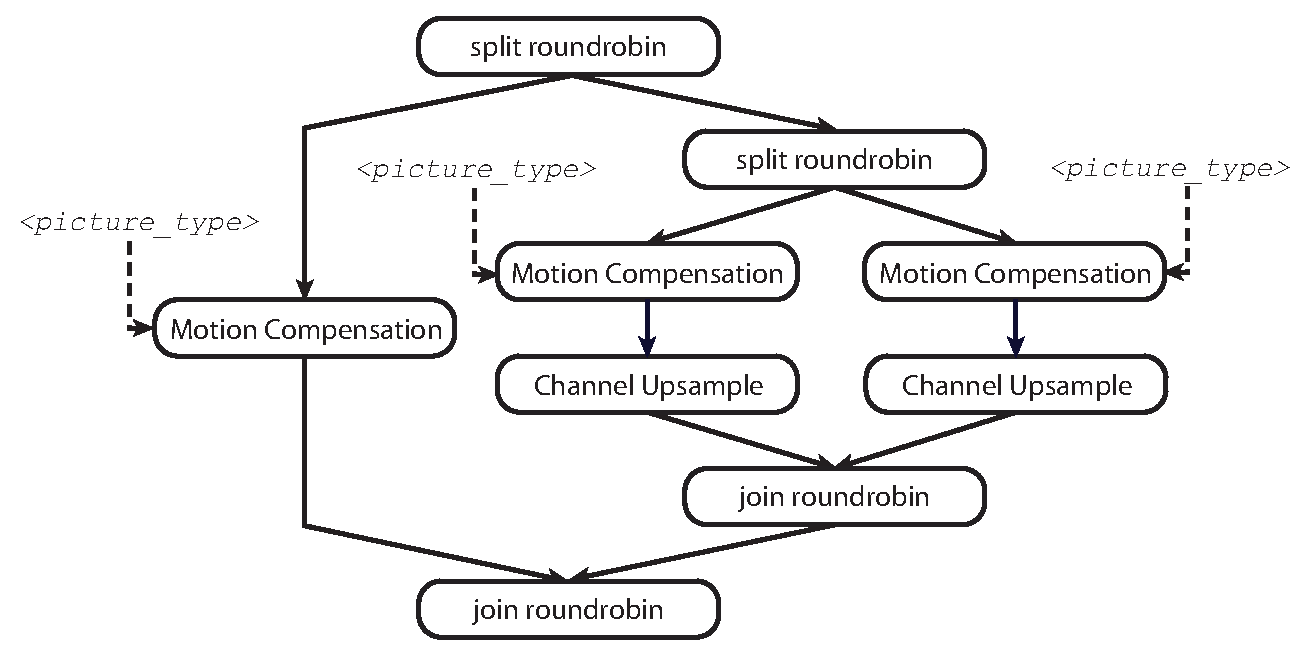
\includegraphics[scale=0.5, angle=0]{./chroma_splitjoin.eps}
    \caption{Modified subgraph for handling 4:2:0 and 4:2:2 chroma formats.}
    \label{fig:chroma-format-graph}
  \end{center}
\end{figure}

A noteworthy aspect of the StreamIt implementation is its
malleability. I illustrate this by outlining how the decoder
implementation is modified to support both 4:2:0 and 4:2:2 chroma
formats (see Section~\ref{section:picture_decomp}). 
The conceptual difference between chroma formats is merely a change in
downsampling ratio. The implementation difference is that the 4:2:0 format
represents a macroblock with six blocks, and the 4:2:2 with 8 blocks. This
change affects the data rates, and the data splitting ratios between color channels. 
In the C reference code, the change requires adjustments to buffer sizes, array lengths, array
indices, loop bounds, and various pointer offsets. The reference implementation
uses a \textbf{chroma flag} to dictate control flow and alternate
index/offset calculations in 43 locations in the code. As an example,
Figure~\ref{fig:chroma-format-code-C} shows a code fragment from the
\texttt{form\_prediction} routine in
\texttt{recon.c}. The function calls a
subroutine to perform the motion compensation on each of the three
color channels, passing in array offsets to a global array holding the
data. Lines 4-6 adjust values used for address calculations to handle
the 4:2:2 and 4:2:0 chroma formats, and lines 7-9 provide additional
adjustments for the 4:2:0 format. While these offset adjustments are
necessary in C, they are difficult for programmers and make the code
hard to understand.

In StreamIt, I modified 31 lines and added 20 new lines to support
the 4:2:2 format. Of the 31 modified lines, 23 were trivial changes to
introduce the chroma format as a stream parameter. The greatest
substantial change was to the color channel splitter, previously
illustrated on line 17 of Figure~\ref{fig:dec-with-code}. In the case
of a 4:2:2 sampling rate, the chrominance data, as it appears on the
input tape, alternates between each of the two chrominance
channels, as previously shown in Figure~\ref{fig:chroma_format}.
Thus, a nested splitjoin is used to properly recover the
chrominance channels. 

The code for the old splitjoin before the chroma format
support modifications is shown in 
Figure~\ref{fig:chroma-format-code-streamit-previous}.
The code for the new splitjoin is shown in 
Figure~\ref{fig:chroma-format-code-streamit} and
illustrated in Figure~\ref{fig:chroma-format-graph}.  
In the StreamIt code, the chroma
format explicitly dictates control flow in only 9 locations. Of
course, chroma format changes have effects on scheduling 
and buffer management, but this is transparent to the programmer.

\section{Hierarchical Construction vs Functional Calls}
\label{sec:hier}

Preserving the block structure in the program definition is important for
programmer productivity and maintaining code malleability. 
Figure~\ref{fig:call-diagram}
shows what happens to the block diagram in a traditional language. This figure
represents a simplified call trace for the MPEG-2 decoder in C. 
Note that each component must be wrapped in loops determining the exact number 
of iterations the component must run to fully decode a picture or video. 
Data is stored in global buffers and addresses to these buffers are passed between
functions, so the code structure fails to reflect the actual movement of data.
Finally, notice that the functions for parsing, motion compensation, and spatial decoding are
intermixed in the code for performance reasons.
The StreamIt compiler can interleave the phases of execution to provide performance
but this does not require the programmer to mix functional code.

\begin{figure}[h]
  \begin{center}
    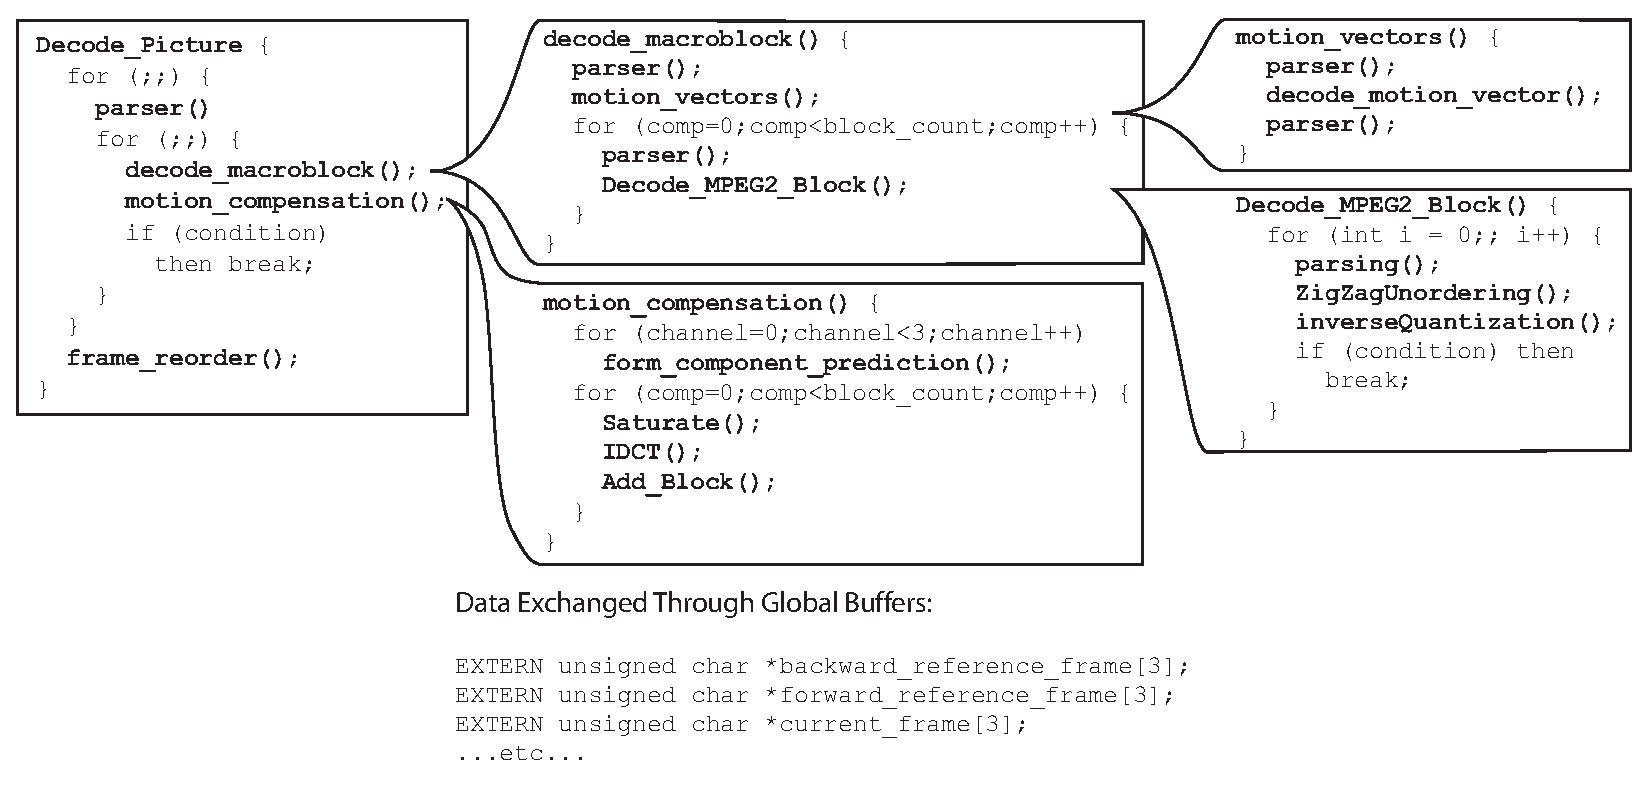
\includegraphics[scale=0.5, angle=0]{./call_diagram.eps}
    \caption{Simplified call-trace diagram for C decoder.}
    \label{fig:call-diagram}
  \end{center}
\end{figure}

\section{Usefulness of Teleport Messaging}
\label{sec:teleport_useful}

Teleport messaging is a useful language construct, as 
demonstrated by its importance in handling control messages 
in the decoder and encoder. 
Figures~\ref{table:enumerate_messages_decoder}~and~\ref{table:enumerate_messages_encoder} 
show the important control parameters that are sent by 
teleport messages in the MPEG-2 codecs. The number of 
subscribers for each message type highlights the usefulness 
of messages. 

\begin{figure}[h]
  \begin{center}
\begin{minipage}{\textwidth}
\renewcommand{\thempfootnote}{
  \arabic{footnote}
}
    \begin{tabular}{|p{1.7in}|l|l|p{0.9in}|p{0.9in}|}
\hline
\textbf{Message Content} & \textbf{Frequency} & \textbf{Regular} & \parbox{0.9in}{\textbf{Number of\\ Subscribers}} & \parbox{0.91in}{\vspace{0.04in} \textbf{Number of\\Subscriber\\Types} \vspace{0.04in}} \\
\hline
quantization scale code & macroblock & no & 2 & 2 \\
quantization tables & video & yes & 2 & 2 \\
macroblock type & macroblock & yes & 4 & 2 \\
picture type & picture & yes & 4 & 2 \\
motion vector resets & macroblock & no & 1 & 1 \\
\addtocounter{footnote}{1}
reference pictures & picture & no & many\footnote{One for every block in all color channels over a picture.} & 1 \\
\hline
    \end{tabular}
\end{minipage}
  \end{center}
  \caption{Important control parameters sent through the decoder using teleport messaging.}
  \label{table:enumerate_messages_decoder}
\end{figure}

\begin{figure}[h]
  \begin{center}
\begin{minipage}{\textwidth}
  \renewcommand{\thempfootnote}{
\arabic{footnote}
}
     \begin{tabular}{|p{1.7in}|l|l|p{0.9in}|p{0.9in}|}
\hline
\textbf{Message Content} & \textbf{Frequency} & \textbf{Regular} & \parbox{0.9in}{\textbf{Number of\\ Subscribers}} & \parbox{0.91in}{\vspace{0.04in} \textbf{Number of\\ Subscriber\\ Types} \vspace{0.04in}} \\
\hline
quantization scale code & macroblock & no & 2 & 2 \\
quantization tables & video & yes & 1 & 1 \\
macroblock type & macroblock & yes & 4 & 2 \\
picture type & picture & yes & 4 & 4 \\
\addtocounter{footnote}{1}
reference pictures & picture & no & many\footnote{Once for every macroblock in all color channels over a picture.} & 2 \\
\hline
    \end{tabular}
\end{minipage}
  \end{center}
  \caption{Important control parameters sent through the encoder using teleport messaging.}
  \label{table:enumerate_messages_encoder}
\end{figure}

Messaging's impact on programmability is evident by 
considering how the C code exposes control relevant information. 
The C code passes data and control parameters through function 
parameters and a global address space. Figure~\ref{fig:c-arrow-diagram} shows the functional
units in the C decoder\footnote{A functional unit might contain multiple functions with
similar or related behaviors.}, the input bitstream, output video, and the shared 
address space. Arrows represent communication dependencies between the blocks. 
While the C implementation is natural --- for C code --- it would be difficult for a 
programmer or compiler to extract 
parallelism\footnote{Because
the analysis of data access patterns is complicated and 
correctness verification for optimizations becomes impractical, 
a compiler will make a pessimistic decision.}.

\begin{figure}[h]
  \begin{center}
    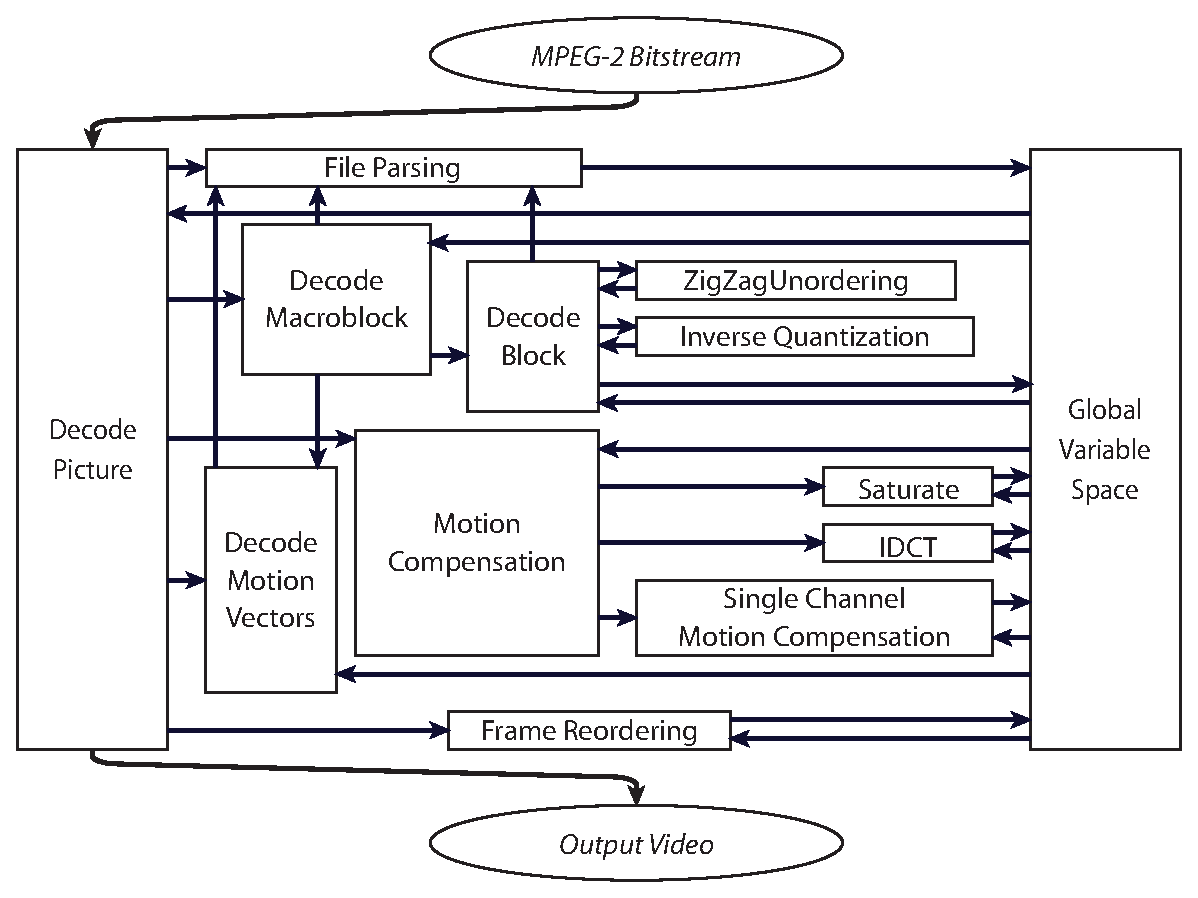
\includegraphics[scale=0.7, angle=0]{./functional_units.eps}
    \caption{Communication dependencies between functional units in the C code.}
    \label{fig:c-arrow-diagram}
  \end{center}
\end{figure}

Teleport messaging provides a point to point connection layer 
which a programmer can emulate in the dataflow layer by 
embedding control parameters in the data channels. While
StreamIt provides the feedback loop construct
to send information upstream, messaging is often more
appropriate for altering upstream state. 

Upstream reference frame passing in the encoder is used as an example. 
A feedback loop structure is impossible here, due to the fact that 
only some pictures should be sent upstream as reference pictures, 
and the information about which pictures to send upstream is not 
available at compile time. This would require the feedback loop to 
process messages regarding picture type and implement a dynamic 
rate splitter and joiner. This is not intuitive to implement, 
nor would it be easy for the compiler to analyze. Without B 
pictures the feedback loop structure needed to ensure that 
each motion estimation filter received the right reference frame 
immediately before the first block of a picture would still be 
non-trivial. Replacing the messaging scheme with a feedback loop 
would also effectively require the motion estimation filters to 
operate at a picture granularity, since each work execution 
would receive a reference picture, and this would limit 
parallelism by preventing estimation to be expressed at a block 
granularity. 

This chapter has given specific instances of where StreamIt improved
programmer productivity. Personal qualitative observations on the entire
implementation process are also pertinent. I found programming in StreamIt
to be very intuitive.
MPEG-2 decomposed naturally into concise independent filters. 
Filters make a program more modular than equivalent C code, 
which made it easy to change the encoder and decoder
stream graphs as my understanding of MPEG-2 improved. For the purposes
of correctness verification and performance comparisons it was much easier
to extract functional units from the StreamIt code than the C code.


\chapter{Expressing Parallelism}
\label{chapter:exposing_parallelism}

Multimedia codecs such as MPEG-2 demand high performance because of throughput
requirements. An online encoder or decoder must be capable of realtime performance,
which can be as high as 60 fps. An offline encoder is less constrained but minimizing
total runtime is still a concern. Since traditional CPU clock scaling has ended,
meeting throughput demands requires parallel scalable implementations. 
Critical to these implementations is the compiler's ability to detect parallelism
in a program specification. 
This section examines how parallelism was successfully 
realized in the MPEG-2 codecs and how the StreamIt language made this task easy. The 
parallelism discussed in this section is exposed through the stream graph 
topology rather than by changing any underlying algorithms. This section ignores 
parallelizing MPEG-2 codecs across GOPs; since GOPs are coded independently, 
this is embarrassingly parallel and trivial. I also include proof of 
concept results showing that the StreamIt implementation scales on multicore
architectures.

\section{Splitjoins Express Data Parallelism}

One particularly noteworthy aspect of splitjoins is the ability to define 
their internal topology using the for-loop construct. The for-loop, unrolled at 
instantiation time, makes the degree of parallelism and the stream topology
itself parameterizable. 
This feature makes it easy for the programmer to concisely express a data parallel 
computation. The code responsible for channel upsampling, shown in 
Figure~\ref{fig:upsamplecode}, expresses a massively data parallel computation in 
this way. 

\section{Hierarchical Streams Expose High Degrees of Parallelism}
\label{sec:2d_dct}

\begin{figure}[h]
  \begin{center}
    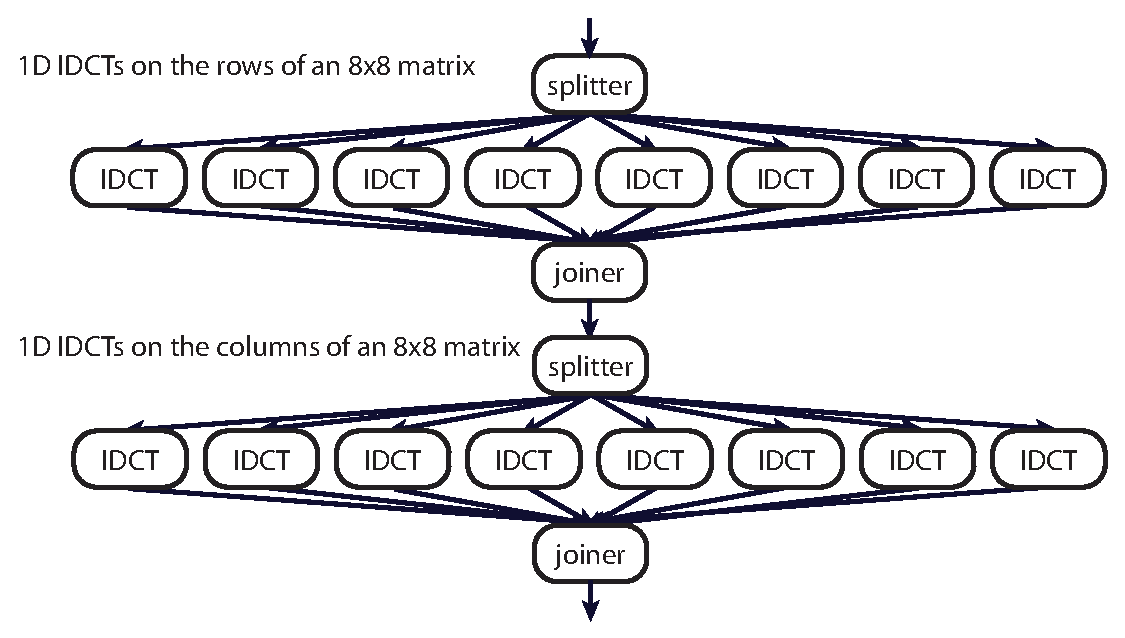
\includegraphics[scale=0.6, angle=0]{./dct_block.eps}
    \caption{Subgraph for a fine grained 2D inverse DCT.}
    \label{fig:decoder-sj-graph}
  \end{center}
\end{figure}

\begin{figure}[h]
  \begin{center}
    \begin{minipage}{4in}
      \begin{small}
        \begin{verbatim}
float->float pipeline IDCT_2D(int N) {
    // perform N 1D-IDCTs in parallel in the X direction
    add splitjoin {
        split roundrobin(N);
        for (int i = 0; i < N; i++)
            add IDCT_1D(N);
        join roundrobin(N);
    }
    // perform N 1D-IDCTs in parallel in the Y direction
    add splitjoin {
        split roundrobin(1);
        for (int i = 0; i < N; i++)
            add IDCT_1D(N);
        join roundrobin(1);
    }
}

float->float filter IDCT_1D(int N) {
    float[N][N] coeff = { ... };
       
    work pop N push N {
        for (int x = 0; x < N; x++) {
            float product = 0;
            for (int u = 0; u < N; u++)
                product += coeff[x][u] * peek(u);
            push(product);
        }
        for (int x = 0; x < N; x++) pop();
    }
}
        \end{verbatim}
      \end{small}
    \end{minipage}
  \end{center}
  \caption{StreamIt code for the fine grained 2D inverse DCT subgraph.}
  \label{fig:decoder-sj}
\end{figure}

\begin{figure}[h]
  \begin{center}
    \begin{minipage}{4in}
      \begin{small}
        \begin{verbatim}
// global variable
float coeff[64] = { ... };
      
void IDCT_2D(float* block) {
    int i, j, u;
    float product;
    float tmp[64];
        
    // 1D DCT in X direction
    for (i = 0; i < 8; i++)
        for (j = 0; j < 8; j++) {
            product = 0;
            for (u = 0; u < 8; u++)
                product += coeff[u][j] * block[8*i + u];
            tmp[8*i + j] = product;
        }

    // 1D DCT in Y direction
    for (j = 0; j < 8; j++)
        for (i = 0; i < 8; i++) {
            product = 0;
            for (u = 0; u < 8; u++)
                product += coeff[u][i] * tmp[8*u + j];
            block[8*i + j] = product;
        }
}
        \end{verbatim}
      \end{small}
    \end{minipage}
  \end{center}
  \caption{C code for 2D inverse DCT calculation using two 1D transforms.}
  \label{fig:idct_creference}
\end{figure}

Hierarchical constructs provide a convenient and natural
way to represent parallel computation. 
Figure~\ref{fig:decoder-sj-graph} shows a parallel
implementation of the 2D IDCT using 1D IDCTs. This
implementation is both data parallel (within the rows and columns) and
pipeline parallel (between the rows and columns). 
The StreamIt code for this 2D IDCT appears in Figure~\ref{fig:decoder-sj}.
A straightforward C implementation of a computationally equivalent
IDCT is shown in Figure~\ref{fig:idct_creference}. Note that
the code structure is similar to the StreamIt version, although it does 
not explicitly expose the parallelism; the compiler must perform loop
and dependency analysis to enable parallelism.
The C code also requires explicit array index management, such as the 
expressions $\texttt{block[8*i+u]}$ and $\texttt{tmp[8*i+j]}$, which are
notably absent in the StreamIt code. 
The splitter and joiner in StreamIt free the programmer from
tedious indexing operations, which also enables the compiler to
understand and optimize the buffer management~\cite{sermulins05lctes}.
The StreamIt implementation is also parameterized such that it is
trivial to adjust the size of the IDCT.

\section{Parallelizing Motion Prediction}
\label{sec:parallelmotion}

Motion prediction, in both the decoder and encoder, represents a significant fraction of the 
computational effort, and is amenable to data parallelism. Because each block in a 
picture has an associated set of motion vectors, motion prediction filters 
express a block-level transformation, and predictions for blocks may be formed in 
parallel. However, the act of forming the prediction requires a filter have access to 
full reference pictures. A parallel implementation of motion prediction will either lead 
to redundant copies of the reference pictures or the necessity for motion prediction 
threads to share a global read only memory space where the reference pictures can be stored. 
A parallel motion prediction algorithm is easy to express in StreamIt and exposes the 
necessary information so that the compiler can provide a shared-memory storage for the 
reference pictures.

\begin{figure}[h]
  \begin{center}
    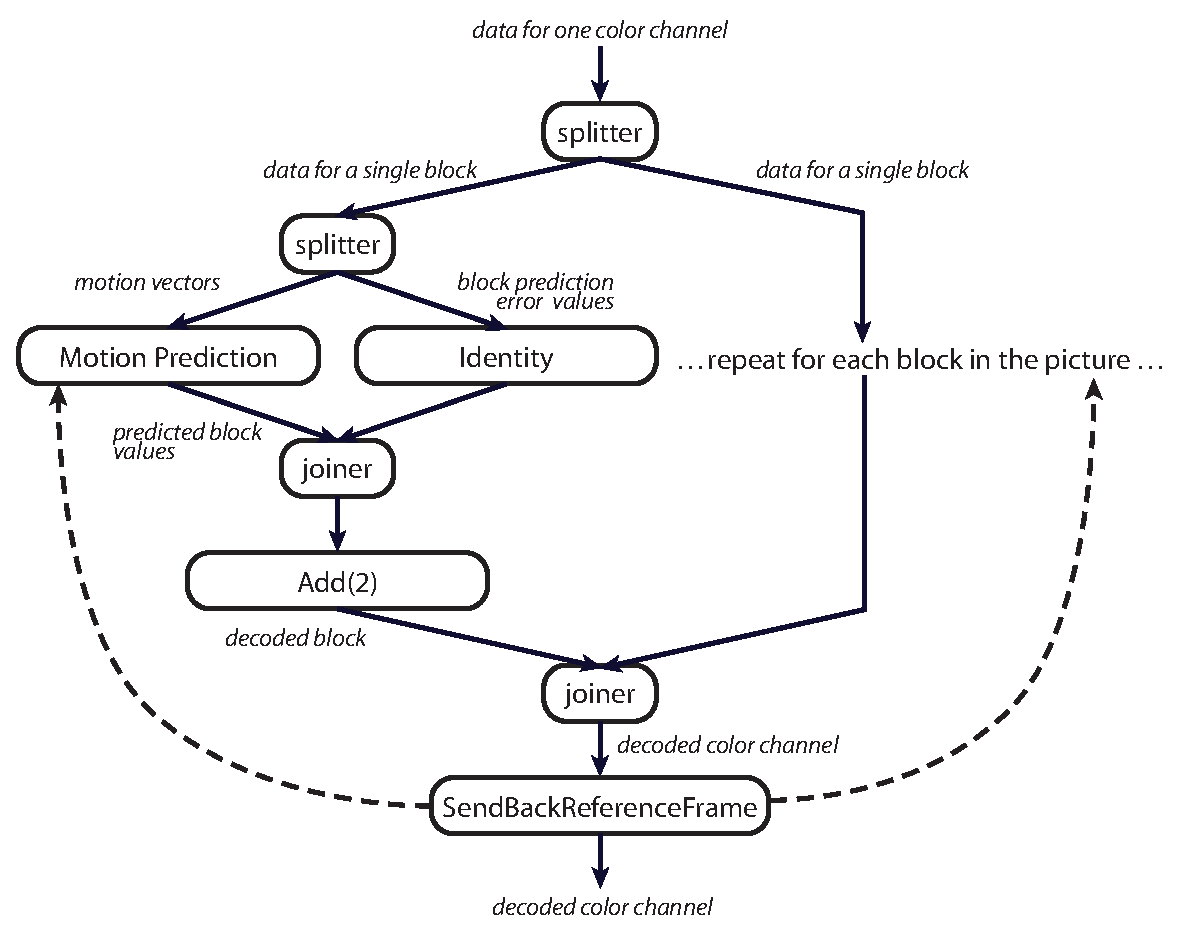
\includegraphics[scale=0.7, angle=0]{./motion_compensation.eps}
    \caption{Stream topology for motion compensation of a single color channel.}
    \label{fig:motion_prediction_parallel}
  \end{center}
\end{figure}

Figure~\ref{fig:motion_prediction_parallel} shows the StreamIt pipeline responsible for 
motion compensation of a single color channel in the decoder. All blocks in a given 
picture are motion predicted in parallel, with a set of block prediction error values 
and motion vector information sent to each motion prediction filter. Each data set then 
has its block coefficients (which need no processing) and the motion vectors splitup, 
sending the motion vectors to the filter that actually does the work of computing the 
predicted block using the motion vector offsets. The predicted block output is added 
to the block prediction error to form the original block, and all blocks are 
interleaved in the data streams. The final filter in the stream graph is responsible for 
communicating this fully decoded picture back to the motion prediction filters. It 
does this by sending upstream messages containing the reference picture data.

Note the cleanliness of this parallel implementation: 
a programmer could manually change the number of blocks 
decoded in parallel and similarly, the compiler can 
automatically fuse filter instances to match the target 
hardware. 
Note also that the reference pictures needed 
by the motion compensation filter and the picture type 
data needed by both the motion compensation and 
reference frame sending filters are naturally expressed using 
messaging. Finally, note that the motion compensation filters
only need to form predictions using their available reference
pictures and a separate filter can make sure they access
the correct references.

As mentioned previously, the one potential drawback of this
scheme would be if each instance of the motion prediction 
filter required its own instance of the reference picture 
data. However, a simple optimization allows the compiler to 
detect that these motion prediction filters only use these 
reference pictures in a read-only context and they may be 
stored in a global address space. Suppose that a filter 
receives a message containing a nugget of data $X$. If a 
compiler can detect that the filter never modifies $X$, 
it can place a copy in a shared memory space and give the 
filter a reference to $X$. Whenever a new message is 
received, it simply gives the filter a new reference to the 
data in a different part of the shared memory space. If 
a filter modifies $X$ or the compiler cannot detect 
that the filter uses $X$ immutably, it must give the 
filter a copy of the message in its own address space. Some 
kind of reference count or garbage collection mechanism 
must be associated with data stored in the global space 
so that the memory can be freed or reused once no filters 
can access the data.

The read-only analysis and associated space saving 
optimization can be performed by the compiler automatically. 
This enables program implementations to use a global 
reference space, even though the language need not provide 
this feature. I have tested a prototype of this optimization 
in the StreamIt Java library, where garbage collection is 
easily handled, and verified that it works.

\section{Improving Decoder Parallelization}
\label{section:super_parallel}

Most MPEG-2 decoder implementations make spatial decoding 
precede temporal decoding, but nothing in the specification 
or decoding algorithms require this. To achieve a higher degree of 
parallelization, one would want to generate the predictions for a 
block in parallel with the spatial interpretation of the block 
coefficients. This has been tried with success in a hardware based 
implementation~\cite{schneider99spec}. Only near the final output 
stage must the prediction and spatial data be summed and the output 
generated.

\begin{figure}
  \begin{center}
    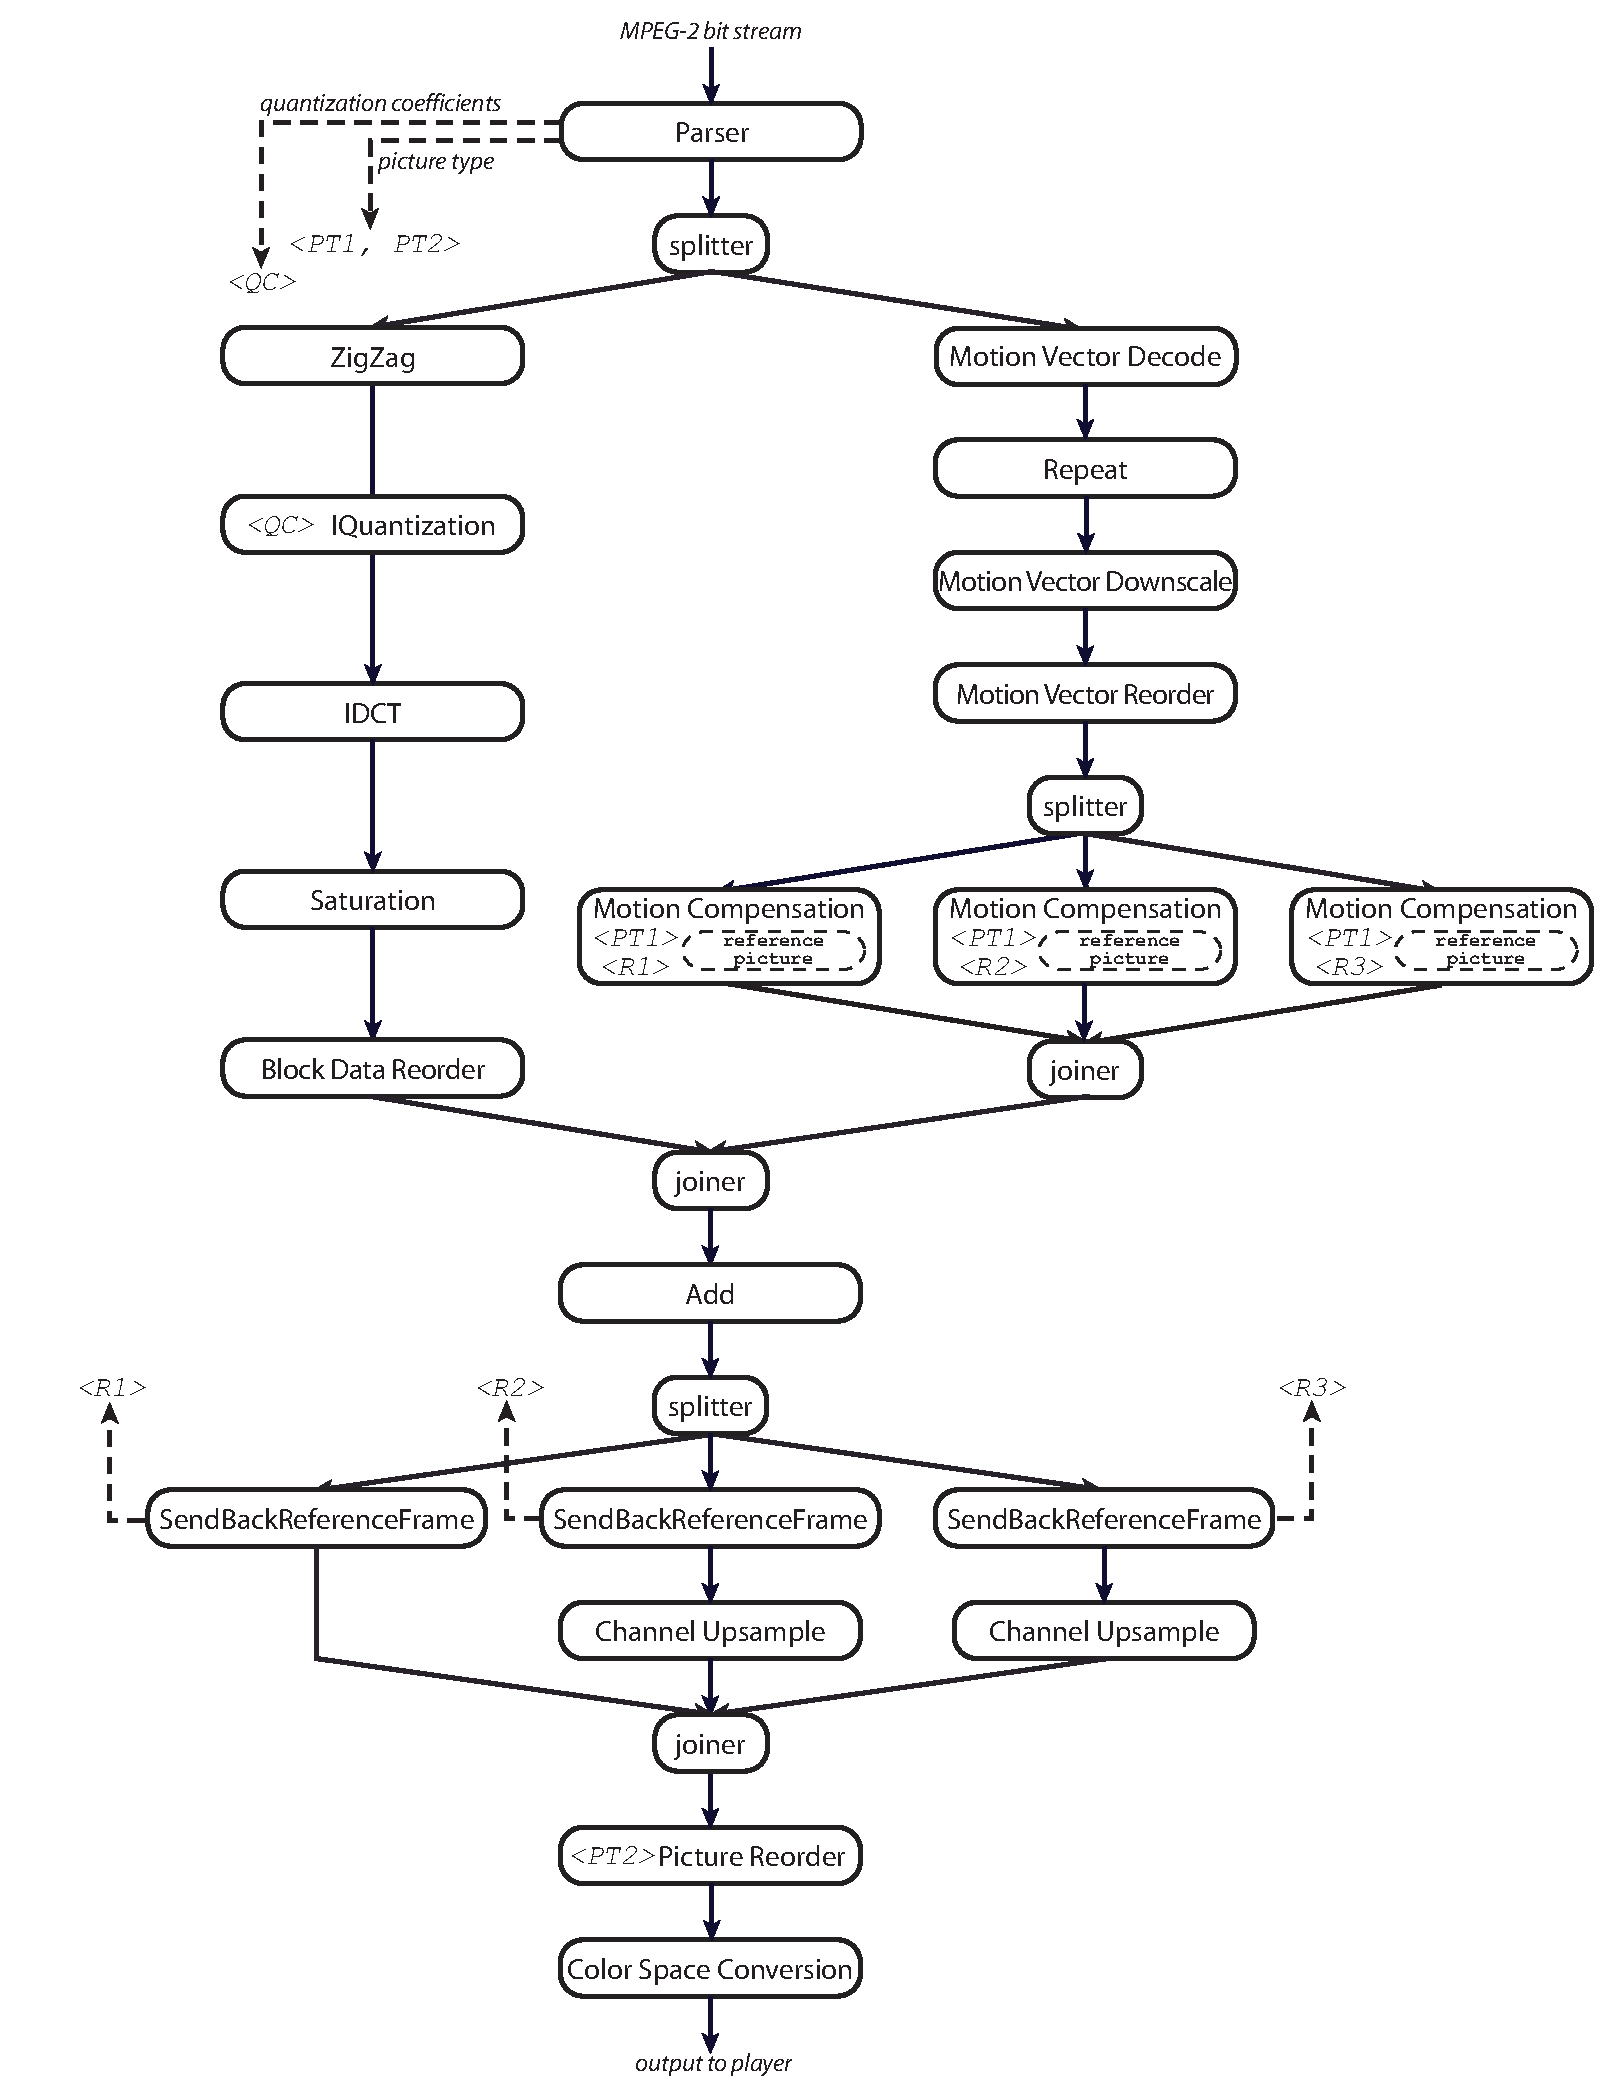
\includegraphics[scale=0.40, angle=0]{./decoder_total_parallelization.eps}
    \caption{Exposing parallelism between spatial and temporal decoding in an MPEG-2 decoder.}
    \label{fig:total_parallelization_vs_old_way}
  \end{center}
\end{figure}

I previously showed a block diagram for the MPEG-2 decoder 
in StreamIt (in Figure~\ref{fig:dec-with-code}). This diagram 
represents both a straightforward block specification and a program 
definition derived from the specification.  
Figure~\ref{fig:total_parallelization_vs_old_way} shows 
an alternative block diagram for an MPEG-2 decoder. This 
alternative diagram shows a block diagram that an MPEG-2 expert will decide 
upon\footnote{The original diagram represents the program structure 
I chose a month after originally familiarizing myself with the 
MPEG-2 specification. The new diagram represents the program 
structure I chose 8 months later after extensive familiarity 
with the specifications and implementations.}. These two block 
diagrams contain the same functional transformations. For an 
ideal language, a clean and malleable implementation of the 
original block specification in Figure~\ref{fig:dec-with-code} 
could easily be modified to expose the greater degree of 
parallelism present in the expert's block structure in 
Figure~\ref{fig:total_parallelization_vs_old_way}.

Because StreamIt preserves block structure in the program 
definition this transformation is easily accomplished. I have 
implemented the alternate decoder, using exactly the same 
filters as those used in the original decoder implementation. 
These two implementations are functionally equivalent, 
generating the same output across test cases. The only 
changes in the code are to the nested hierarchical container 
topologies that dictate the decoder stream graph. The ease 
with which a programmer can expose greater parallelism by 
merely changing the stream topology points to the 
usefulness of stream based languages for parallel program 
implementations.

\section{Performance Results}

This section provides performance results showing how StreamIt 
enables a compiler to provide scalable performance on MPEG-2 
codec implementations. A need for new language features previously 
mentioned in this thesis prevents the compilation of a full 
decoder or encoder\footnote{An intermediate Java library output 
from the compiler allows me to verify correctness of StreamIt code. This target is 
not performance oriented.}. 
Execution and evaluation of the complete MPEG-2 decoder and encoder stream graphs 
is a current focus of the StreamIt group.
Here I consider the spatial decoding subgraph, 
which represents up to a third of the total computation
in the decoder~\cite{iwata98coarse}.
I have extracted the 
spatial decoding code from the StreamIt and C decoder implementations
so that it can be compiled and run on a performance oriented target.

\begin{figure}[h]
 \begin{center}
  \begin{tabular}{|l|c|c|}
\hline
Granularity & Nodes in IDCT & Nodes in Graph\\
\hline
Coarse & 2 & 8 \\
Intermediate & 11 & 17\\
Fine & 20 & 26\\
\hline
  \end{tabular}
  \end{center}
 \caption{Three versions of the spatial decoding stream graph and their granularities.}
 \label{table:decoding_graphs}
\end{figure}

I use three versions of the StreamIt spatial decoding stream graph with
differing granularities. The granularities are changed by altering the subgraph
for the 8x8 IDCT. Figure~\ref{table:decoding_graphs} lists the number of nodes
(filters, splitters, and joiners), contained in the stream graph for each
of the three versions.
Each version contains \texttt{Source}, \texttt{ZigZag}, 
\texttt{InverseQuantization}, \texttt{Saturation}, \texttt{MismatchControl}, and
\texttt{Sink} filters. The coarse grained IDCT uses 2 filters for the IDCT: 
a \texttt{Rows\_iDCT} and a \texttt{Columns\_iDCT} filter. The fine grained
IDCT is expressed with 16 1D IDCTs and two splitjoins as described 
in Section~\ref{sec:2d_dct}. 
The intermediate IDCT uses the coarse \texttt{Rows\_iDCT} filter for the row
transformation and the fine grained column transformation with 8 1D IDCTs.

The performance evaluation is carried out on the Raw architecture
\cite{taylor:micro:2002, taylor:isca:2004}.
The Raw architecture is representative of the industry shift to multicore
embedded architectures, currently manifested in emerging architectures
such as the Intel Duo, AMD Opteron, and IBM Cell processors.
Raw is a wire-exposed multicore architecture which contains a 2D array of identical,
programmable tiles 
and supports instruction, data, thread, and pipeline parallelism. 
Each tile has a compute processor and a switch processor that
manages communication. The compute processor is composed of an eight-stage
in-order single-issue MIPS-style processor, a four-stage pipelined floating point unit,
a 32kB data cache, and a 32kB instruction cache. 
Tiles are connected by a FIFO queue 
with a 3 cycle near neighbor latency. This interconnect
network provides a mechanism for filters to communicate quickly with each other.
The current Raw prototype is a chip with 16 tiles running at 425Mhz. 
For this thesis, results are gathered using
a cycle-accurate simulator~\cite{taylor:isca:2004} that can model tile configurations
with size
1, 4 (2x2 grid), and 16 (4x4 grid). 

\begin{figure}[p]
  \begin{center}
    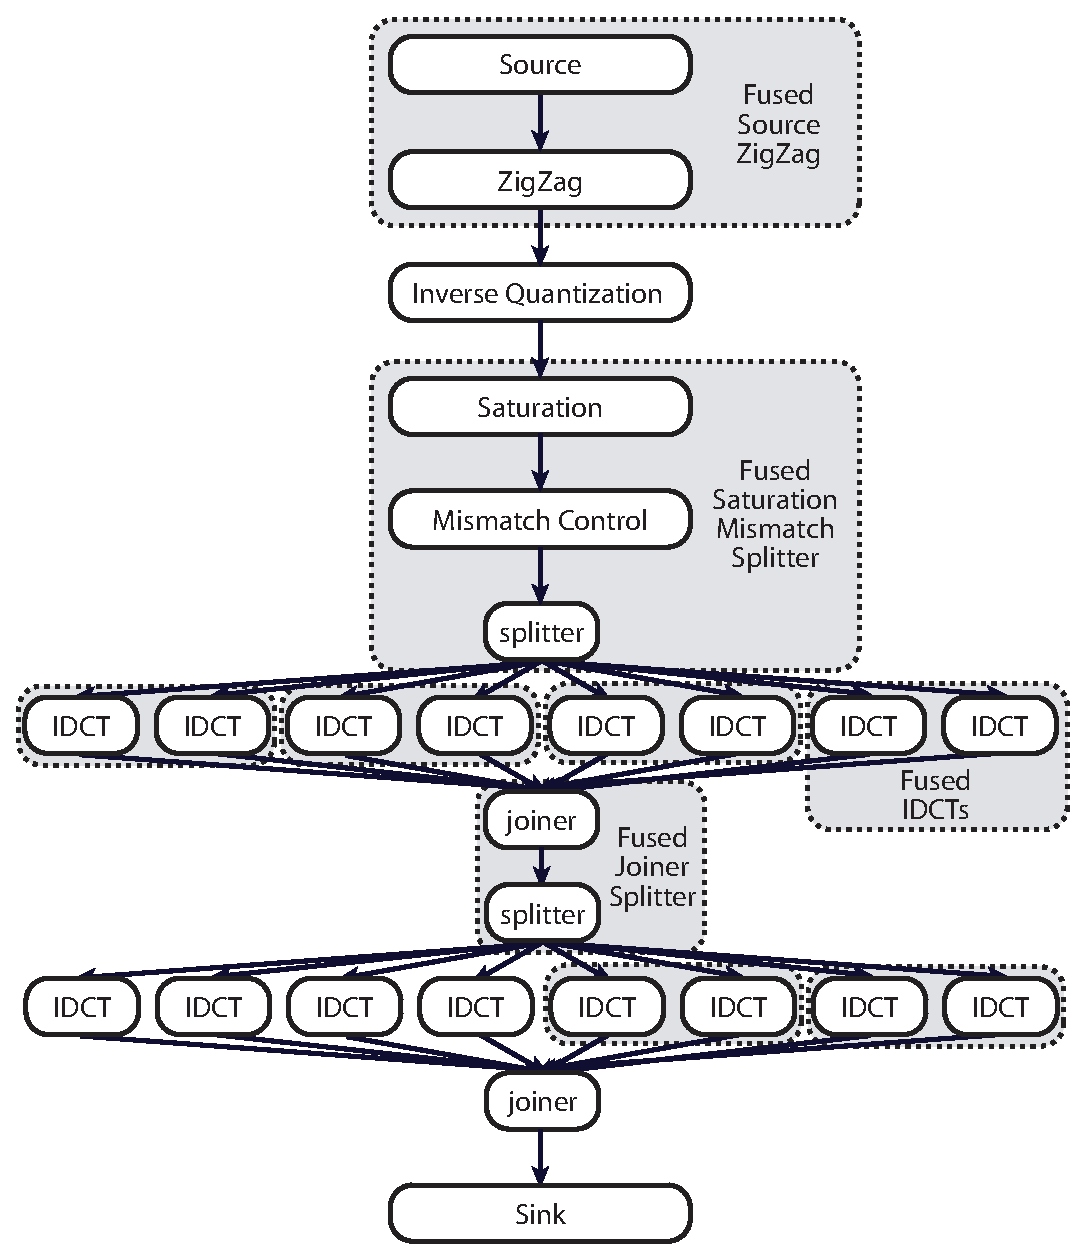
\includegraphics[scale=0.5, angle=0]{./partition.eps}
    \caption{Partitioning the spatial decoding stream graph for 16 tiles of Raw.}
    \label{fig:partition}
  \end{center}
\end{figure}

\begin{figure}[p]
  \begin{center}
    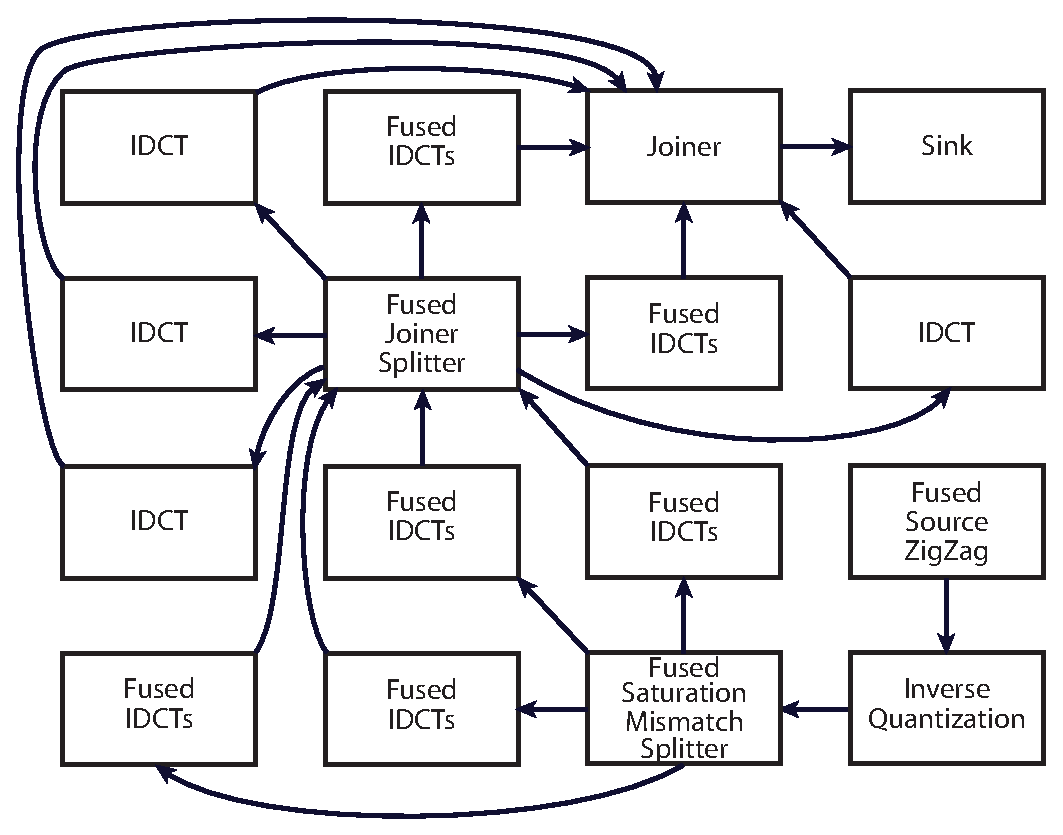
\includegraphics[scale=0.5, angle=0]{./layout.eps}
    \caption{Layout of the fine grained spatial decoding stream graph on the Raw chip.}
    \label{fig:layout}
  \end{center}
\end{figure}

The StreamIt code was compiled to Raw with the StreamIt 
space multiplexing compiler
\footnote{This compiler will soon be
deprecated in favor of a more advanced space-time multiplexing
compiler described in an upcoming paper~\cite{gordon06asplos} 
from the StreamIt group.}
described in~\cite{gordon02asplos}.
The code was compiled at an \texttt{-O1} optimization level, 
which performs loop unrolling by a factor
of 16, scalar replacement, and aggressive constant propagation. 
The StreamIt compiler focusses on achieving
performance by enabling scalable execution on
many tiles. Using the parallelism explicit in the stream graph the compiler
automatically performs task partitioning and layout.
An application should achieve significant speedups as the number of tiles increases.

A brief example illustrating
scheduling and layout follows.
Figure~\ref{fig:partition} shows how the StreamIt
compiler partitions the fine grained 
spatial decoding stream graph for a Raw configuration with 16 tiles.
The compiler adjusts the stream graph granularity by combining
nodes to eliminate buffering between nodes on the same tile. 
The dotted lines in the figure show which nodes in the stream graph have been fused.
After fusion is complete there are the same number of nodes and tiles 
in the stream graph. Figure~\ref{fig:layout}
shows the compiler's layout decision for these nodes on the Raw hardware.

\begin{figure}[t]
  \begin{center}
    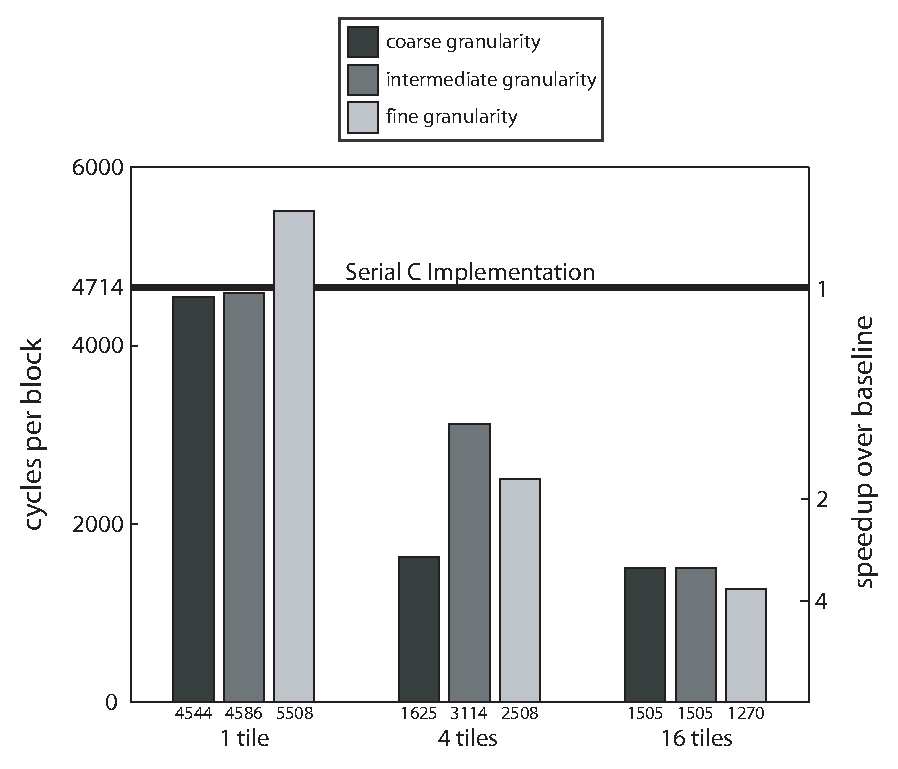
\includegraphics[scale=0.7, angle=0]{./performance_graph.eps}
    \caption{Scalability of StreamIt spatial decoding pipeline against single tile C baseline.}
    \label{fig:performance_results}
  \end{center}
\end{figure}

Figure~\ref{fig:performance_results} shows results for execution of 
the spatial decoding stream graph at three granularities.
The baseline is
the C reference code running on a single tile. 
The C code was compiled with a Raw port of the \texttt{gcc} compiler,
which performs register allocation and list scheduling.
A compiler has a difficult time extracting parallelism from single threaded C code
(hence the need for new programming models); in StreamIt the parallelism
is explicit, so we show performance numbers for multi-tile 
configurations as well. 

Single tile StreamIt performance is roughly equivalent to the
single tile C code. Small variations are explained
by compiler decisions about how to fuse all the filters together. 
When the tile size increases to 4, all versions of the StreamIt
code significantly outperform the C implementation. While 
the coarse grained
version of the StreamIt code outperforms the more fine grained
implementations, an analysis of the compiler's layout decisions suggests
that this result is somewhat anomalous: the compiler is 
getting exceptionally lucky with load balancing. The intermediate
and fine grained versions are more prototypical.
At 16 tiles performance of all stream graphs 
again improves significantly. One 
sees the general trend that decreasing the granularity of
the program enables the compiler to make better layout
decisions and provide higher parallel performance. The best 
performance comes from a fine-grained implementation 
operating on 16 tiles.

\documentclass[11pt]{article}

\usepackage{cite}
\usepackage[margin=1in]{geometry}
\usepackage{palatino}
\usepackage{url}

% Abstract formatting:
\def\class#1{\texttt{#1}}


% Print acronyms in small caps.
\def\cfg{\textsc{cfg}}
\def\dsp{\textsc{dsp}}
\def\fortran{\textsc{fortran}}
\def\ir{\textsc{ir}}
\def\Ir{\textsc{Ir}}
\def\mips{\textsc{mips}}
\def\mit{\textsc{mit}}
\def\opi{\textsc{opi}}
\def\raw{\textsc{raw}}
\def\scale{\textsc{scale}}
\def\sir{\textsc{sir}}
\def\ssa{\textsc{ssa}}
\def\Ssa{\textsc{Ssa}}
\def\stair{\textsc{stair}}
\def\Stair{\textsc{Stair}}
\def\suif{\textsc{suif}}
\def\Suif{\textsc{Suif}}
\def\suifvm{\texttt{suifvm}}
\def\vliw{\textsc{vliw}}
\def\vm{\textsc{vm}}
\def\xml{\textsc{xml}}
\def\Xml{\textsc{Xml}}
\def\machsuif{Machine \suif}

% Predefine useful email addresses.
\urldef\dmazemail\url{dmaze@cag.lcs.mit.edu}

\title{Commentary on \stair}
\author{David Maze\\\dmazemail}

\begin{document}

\maketitle

\begin{itemize}
\item 2.3, 2. Seems to me like types would still be useful --- might
  want a "bit" in addition to int and float?  (I don't know, if we
  ever generate hardware from low-level IR, for example.) But required
  bitwidth for everything does seem like overkill.  [Bill]
  
\item Variables.  Do we want to distinguish SSA by number or name?
  Seems like if you want to get a new SSA variable, you might just
  want to get a fresh name instead of finding what the current free
  number is for that variable.  [Bill]

  \emph{SSA-by-number means that it's easier to collect together
    different parts of the same variable without copying values around
    when doing register allocation.  ---dzm}
  
\item The array addressing case.  Wouldn't it be much easier for a
  lower layer to convert a single instruction to multiple instructions
  instead of the other way around? Seems like the store should be the
  most general, high-level version in the common layer.  So I'd vote
  for store-with-offset instead of doing the add of the address in the
  VM.  [Bill]
  
\item Branching.  I'm a little confused about why the insert
  conditional branch, etc., is in the Backend interface.  Isn't there
  a vm-level concept of branches?  Are all branches machine-specific?
  Why aren't they just like other instructions?  (Or you're saying
  that at the vm level, all branches are just implied by the control
  flow graph?  Still there needs to be some instruction for
  designating which path to take, I guess.)  [Bill]
  
  \emph{My intent was that everything would stay in \cfg{} form until
    the latest possible moment.  So all of the control flow, including
    conditional and unconditional branches, is in the \cfg.  This
    isn't necessarily ideal; we might want to break the \cfg{} around
    calls, for example.  ---dzm}
  
\item 4.4 Symbols --- are "variables" the same as temporary operands
  in the low-level \ir?  when you say "symbols and registers, but
  nothing else, have types" --- what's the "else"?  I think the
  temporaries in the low-level IR should have types as well.  [Bill]
  
  \emph{When a temporary is generated, it gets a slot in the symbol
    table, so it becomes a normal variable.  The "else" includes
    immediates (implicit integer or float type) and memory references
    (where you probably care).  The immediates are the thing that are
    a big pain with typing in \machsuif.  ---dzm}
  
\item I don't think don't think edge should be inner class of block,
  if that's what you were really intending.  (Passes might want to
  know about edges.)  [Bill]
  
  \emph{That is what I was intending.  That can be changed.  There's
    some concern about the names I'm using being pretty generic ones,
    though; I might use ControlEdge over an unqualified Edge.  ---dzm}
  
\item I think a major open question is whether or not the "low-level
  IR" is structured.  At one point (around StreamIt Fun Day '02) we
  were talking that there should be an architecture-independent
  equivalent of the "flat graph" that Mike Gordon currently uses in
  the Raw backend.  Maybe \stair{} is independent of this decision
  (\stair{} code could appear either in \sir{} function bodies, or in
  some low-level graph function body) but when we're building the
  infrastructure, I think it'd be good to introduce the generic
  unstructured graph at the same time.  Maybe Gordo can help define
  this -- or could just distill it from his Raw code.  [Bill]

\item Shouldn't there be phi nodes?  [Bill, paraphrased]

  \emph{Oh yeah, that didn't make it into the original document.  Each
    block should have a list of variables and associated \ssa{}
    numbers live on entry and exit.  Then, for each variable, either
    the \ssa{} number is identical to all of the previous blocks, or
    it's different from all of the previous blocks and an implicit phi
    function exists.  ---dzm}
  
\item Is there any value in having the \cfg{} and the textual sequence
  of instruction just be redundant views of the same thing?  Michal
  was describing algorithms where you just loop through a linear
  stream of instructions and follow the branches for a simple way of
  doing things.  I think the same thing could be done through a \cfg,
  but I can't tell if it'd be more cumbersome.  [Bill]
  
\item Perhaps \class{BlockContainer} should be replaced by
  \class{Function}; are there other interesting case of containers?
  [Bill]

\item Probably want more widespread use of annotations.

  \emph{Makes sense.  I'm not sure how much we actually want to
    annotate; annotations on instructions, blocks, and symbols all
    make sense, but on individual operands might be a bit excessive.
    Annotating blocks is also a little risky if blocks are going to be
    repeatedly refactored.  ---dzm}

\item \Suif's approach to types, using explicit bit sizes on types, is
  good.  This implies that a general type-conversion instruction is
  necessary.  Not having types on constants is fine, though.  [Mike K]

\item While control flow graphs can be useful, should they be the only
  representation of the program?  Having a flat graph can be useful.
  [Mike K]

  \emph{After discussion in the meeting, it sounds like people are
    happy if there isn't a hard global invariant that the \cfg{}
    representation isn't a fixed minimal control-flow graph of basic
    blocks.  In particular, Mike is satisfied if the representation
    has a ``flatten'' call that produces a single \class{Block}
    containing all of the code for a function.  In turn, this means
    that branch and label instructions are necessary in the \vm{}
    layer.  Functions to do common \cfg{} manipulations such as
    ``insert a block before this one'' also are important.}

\item \Ssa{} is a bit overrated.  We don't necessarily want to use it
  everywhere, and it's not useful for array references and globals.
  [Everybody]  ``It's fine if it's optional.''

  \emph{The \ssa-with-numbers approach does make \ssa{} pretty
    optional; if you don't want to use the \ssa{} information, you can
    just ignore it.  Since recomputing the liveness information can
    take time and passes might not need it, this means that passes
    using \ssa{} should be forced to recompute the relevant
    information.  Dealing with arrays and globals is an issue,
    though.  ---dzm}

\item The \ir{} has an operand field for predicates; the input \vm{}
  code should be unpredicated, though.

\item Having array and field access instructions in the \vm{} is
  useful for analysis.  It's better to have the instructions and
  dismantle them than to not have the instructions and be forced to
  reconstruct the information.  [Mike K]

\item \Suif{} has ``registers'' and ``memory'', but no ``symbols''.
  Registers in this world can be virtual registers, or can be bound to
  a hard register.  This means that the symbol table hierarchy can be
  eliminated, or at least reduced.  It also simplifies generating
  temporaries.  [Mike K]

  \emph{I suspect the concept of a symbol is still useful; if nothing
    else, you might want to annotate it for alias analysis.  At this
    \ir{} level, we can deal with field variables by putting them in a
    structure that's a function parameter.  This just leaves globals,
    which fall into the ``memory'' world.  I'm fine with dumping
    symbol tables.  ---dzm}

\item Explicit $\phi$-nodes are useful for \ssa.  Without them, it can
  be hard to find the definition(s) for a particular variable.

\item User-level constants should all be put into globals in the
  program, rather than being used as immediates.

\item There should be strong invariants for the \ir{} that passes can
  easily check.  Similarly, there should be coding standards for
  writing passes so that people who aren't us don't screw it up.
  [Mike K]

\end{itemize}
\end{document}


\section{Conclusions \& Future Work}\label{ch:conc}

Streaming languages provide an excellent way to
target new multicore architectures while placing minimal
parallelization burden on the programmer. Multicore architecture such
as Cell that are designed to offer high peak performance are well
suited for streaming applications. This paper described a runtime
framework for streaming applications on multicores consisting of
\emph{i}) a common Multicore Streaming Layer (MSL) that provides
high-level primitives for schedulers, \emph{ii}) an implementation
of the MSL for an existing processor, namely Cell, \emph{iii}) a
lightweight dynamic scheduler for stream graphs, and \emph{iv}) a
static scheduler for stream graphs. The framework greatly
simplifies the task of a streaming language compiler or scheduler.

The real benefit provided by the framework, in particular the MSL
runtime library, is that it allows a scheduler to think directly in
terms of filters and how they are scheduled instead of lower-level
architecture-specific details. It requires far less code to implement
scheduling patterns on top of the library than directly on Cell
hardware for example, and the MSL library also allows far more complex
patterns to be implemented than directly at a lower level.
 The library running the data-parallel
fused FFT benchmark produces a reasonably small amount of overhead
(1.2\%), and the dynamic scheduler running the pipelined version of
the benchmark produces an acceptable amount of overhead (8.6\%).

The MSL library currently provides two orthogonal branches that can be
further developed. First, it is important to reduce the 9\% overhead
observed in the pipelined FFT tests involving the dynamic
scheduler. This overhead is entirely due to the cost of the run list
when many commands are active, and it can probably be significantly
reduced by optimizing library code, although it is also likely that
doing so would make the SPE library implementation, especially the run
list, much more specialized.

In addition, the implementation currently lacks real support for
filters with dynamic rates (i.e. I/O rates that change over time and
across executions)
-- the library simply leaves the
responsibility of tracking rates to the scheduler entirely. Feedback
from the library on how much data filters have produced and consumed
would be very useful for schedulers; ultimately, the library should
have some way of running filters with unbounded dynamic rates. The
latter would require a general mechanism to suspend dynamic rate
filters in the middle of executing their work functions.

The dynamic scheduler can be extended in many directions. The simplest
additions involve adjusting the metric used for selecting filters to
test and improve the performance of the dynamic scheduler as work
becomes more and more imbalanced between filters. In addition, an
important advantage of dynamic scheduling in general is the ability to
react to dynamic rate filters and the runtime distribution of work in
the stream graph; implementing robust support for dynamic rate filters
in the stream graph would drastically increase its usefulness.


%% This defines the bibliography file (main.bib) and the bibliography style.
%% If you want to create a bibliography file by hand, change the contents of
%% this file to a `thebibliography' environment.  For more information 
%% see section 4.3 of the LaTeX manual.
\bibliography{main}
\bibliographystyle{plain}


%% ALWAYSCHECK - all figs and citations match, all sections match, all references match
%% ALWAYSCHECK - MPEG and StreamIt terms first encountered - bold or italics? make sure it's consistent everywhere
%% ALWAYSCHECK - correct grammar (naked this, which/that, etc)
%% ALWAYSCHECK - compensation vs estimation vs prediction

\end{document}

